\date{}
\title{}
\date{}
\begin{document}
\begin{frame}
    \titlepage
\end{frame}
\input{../common/listingsLib}
\newcommand{\z}[2]{\only<#1->{\myemph<#1>{#2}}}
\newcommand{\zz}[3]{\only<#1-#2>{\myemph<#1>{#3}}}
\newcommand{\zzx}[3]{\only<#1-#2>{#3}}
\newlength{\oneZero}
\settowidth{\oneZero}{\small\tt 0}
\newlength{\twoZeroes}
\settowidth{\twoZeroes}{\small\tt 00}

\usetikzlibrary{calc}

\begin{frame}{last time}
    \begin{itemize}
    \item C code and cache misses
    \item handling writes
        \begin{itemize}
        \item Q1: add to cache on write? (write-allocate)
        \item Q2: update next level immediately? (write-back)
        \end{itemize}
    \item dirty bits for write-back
    \end{itemize}
\end{frame}

\begin{frame}{Side notes re caches}
  \begin{itemize}
  \item Multi-level caches
      \begin{itemize}
      \item First-level cache needs to be fast (and thus small) --- 1-2 cycles hit time, so 32-64 KB L1 I/D
      \item But want high capacity!
      \item So today's high-end processors have two levels of cache per core, and then a huge last-level cache shared among the cores
      \item L2 and LLC are shared I/D; L2 is 256KB--1MB; L3 is usu.\ 128--512 MB
      \item Lots of extra hardware tricks to boost hit rate, e.g. prefetching
      \end{itemize}
  \item Cache lookups with virtual or physical address?
      \begin{itemize}
      \item Cache lookup with VA: aliasing among processes!
      \item But indexing using PA must wait for TLB (only an issue for L1)
      \item So index using VA bits (this means all index bits must be confined to page offset), and do TLB lookup in parallel
      \item Then tag check can use PA bits
     \end{itemize}
  \end{itemize}
\end{frame}

\section{TLB}
\input{../vm/twoLevelPtLib}
\subsection{review: page table lookup (1)}
\input{../vm/twoLevelPTAlt}

\subsection{review: page table lookup (2)}
\againframe<7>{twoLevelPtLookup}

\subsection{why cache page table entries?}
\input{../caching/tlbWhy}

\subsection{how TLB fits in page table lookup}
\input{../caching/tlbMulti}

\subsection{how TLBs are organized}

\usetikzlibrary{decorations,decorations.pathreplacing,circuits.logic.US,matrix,positioning}
\usetikzlibrary{circuits.logic.mux}
\begin{frame}[fragile,label=tlbOrg]{TLB organization (2-way set associative)}
\vspace{1cm}
\begin{tikzpicture}[circuit logic US]
\tikzset{
    myline/.style={-latex,thick},
    myline thin/.style={-latex,thin},
    myline bus/.style={-latex,ultra thick},
    myline no arrow/.style={thick},
    offsetColor/.style={color=yellow!30!black},
    tagColor/.style={color=green!60!black},
    tagStoreFill/.style={fill=green!20},
    tagColorFill/.style={tagColor,fill=green!60!black},
    dataColor/.style={color=blue!60!black},
    dataColorFill/.style={tagColor,fill=blue!60!black},
    dataStoreFill/.style={fill=blue!20},
    triangle down/.style = {draw,regular polygon, regular polygon sides=3, shape border rotate=180},
    N/.style={draw=none,fill=none},
}
\matrix[tight matrix,
        nodes={draw,
               font=\small\tt,
               text depth=0.2ex,
               text height=1.4ex,
        },
        row 1/.style={nodes={font=\small\bfseries,minimum height=1cm,text depth=0.6cm}},
        column 1/.style={nodes={text width=1cm,align=center}},
        column 2/.style={nodes={text width=1cm,tagColor,tagStoreFill}},
        column 3/.style={nodes={text width=1.65cm,dataColor,dataStoreFill}},
        column 4/.style={nodes={text width=1cm,dataColor,dataStoreFill}},
        column 5/.style={nodes={text width=1cm,dataColor,dataStoreFill}},
        column 6/.style={nodes={text width=.1cm,draw=none}},
        column 7/.style={nodes={text width=1cm,align=center}},
        column 8/.style={nodes={text width=1cm,tagColor,tagStoreFill}},
        column 9/.style={nodes={text width=1.65cm,dataColor,dataStoreFill}},
        column 10/.style={nodes={text width=1cm,dataColor,dataStoreFill}},
        column 11/.style={nodes={text width=1cm,dataColor,dataStoreFill}},
        ] (cache) {
    valid \& tag \&  physical page \# \& write \& \ldots \& ~ \& valid \& tag \& physical page \# \& write  \& \ldots \\
    |[N]| \ldots \& |[N]| \ldots \& |[N]| \ldots \& |[N]| \ldots \& |[N]| \ldots \& ~ \&
    |[N]| \ldots \& |[N]| \ldots \& |[N]| \ldots \& |[N]| \ldots \& |[N]| \ldots \\
    1  \& 10 \& 0x123 \& 1 \& ~ \& ~ \& 1 \& 11 \& 0x12F \& 1 \& ~ \\
    ~ \&  ~    \& ~     \& ~ \&  ~ \& ~\& ~ \& ~ \& ~    \& ~     \& ~  \\
    |[alias=bottom-validA]| ~ \&  |[alias=bottom-tagA]| ~ \& |[alias=bottom-ppnA]| ~ \& |[alias=bottom-writeA]| ~  \& |[alias=bottom-miscA]| ~ \& ~ \&
    |[alias=bottom-validB]| ~ \& |[alias=bottom-tagB]| ~ \& |[alias=bottom-ppnB]| ~  \& |[alias=bottom-writeB]| ~  \& 
        |[alias=bottom-miscB]| ~\\
};
\begin{scope}[every node/.style={draw,rectangle,dashed,inner xsep=0pt,outer sep=0pt,font=\tt}]
\node (idx) at ([yshift=.75cm,xshift=-.6cm]cache.north west){100};
\node[left=0cm of idx,tagColor] (tag) {11};
\end{scope}
\node[right=0cm of idx,offsetColor,inner xsep=0pt,outer sep=0pt,font=\tt] (po) {010110};
\draw[thick,dashed,-latex] (idx) |- ([xshift=-.25cm]cache-3-1.west) node[near start,font=\small,fill=white,inner sep=2pt,xshift=-.3cm] {index};
\draw[very thick,decorate,decoration={brace,mirror},overlay] ([xshift=-.1cm]cache-2-1.north west) -- ([xshift=-.1cm]cache-5-1.south west);

\draw[thick,dashed,-latex,tagColor] (tag) |- ([yshift=-1cm]cache-5-2.south) coordinate (tag cmp 1);
\draw[thick,dashed,-latex,tagColor] (cache-5-2.south) -- (tag cmp 1);
\draw[thick,dashed,-latex,tagColor] (tag) |- ([yshift=-2cm]cache-5-8.south) coordinate (tag cmp 2)
    node[midway,fill=white] {tag};
\draw[thick,dashed,-latex,tagColor] (cache-5-8.south) -- (tag cmp 2);

\node[right=.25cm of po,inner xsep=0pt,outer sep=0pt] {(program address)};

\draw[very thick,decorate,decoration={brace},overlay] ([yshift=.05cm]tag.north west) -- ([yshift=.05cm]idx.north east)
    node [midway,above,alt=<2>{red},overlay] {VPN};

\draw[very thick,black!80,decorate,decoration={brace},overlay] ([yshift=.05cm]po.north west) -- ([yshift=.05cm]po.north east)
    node [midway,above,font=\small,alt=<3>{red},overlay] {page offset};


\begin{visibleenv}<4>
\node[fit=(cache-3-3) (cache-3-5),inner sep=1pt,red,draw,line width=1pt,label={[fill=white,fill opacity=0.9]north:page table entry}] {};
\end{visibleenv}

\begin{visibleenv}<5>
\node[fit=(cache-3-1) (cache-3-11),inner sep=1pt,red,draw,line width=3pt] {};
\end{visibleenv}
\end{tikzpicture}
\end{frame}
 % FIXME: emphasize that AFTER this is normal cache access

\subsection{exercise: TLB access pattern}
\input{../caching/tlbAccessExPrep}
\input{../caching/tlbAccessEx}

\section{introduction: correctness}
\usetikzlibrary{arrows.meta}
% not fragile to prevent .vrb from referring to wrong thing
\begin{frame}<0>[label=pthreadCreateBrokenP]{a threading race}
\vspace{-.25cm}
\lstinputlisting[
    style=small,
    language=C++,
    moredelim={**[is][\btHL<1|handout:1>]{@1}{1@}},
]{../threads/pthread-create-race-code.c}
My machine: outputs \texttt{In the thread} \myemph{about 4\% of the time}. \\
What happened?
\end{frame}


\begin{frame}<0>[label=pthreadCreateRace]{a race}
\begin{itemize}
\item returning from main \myemph{exits the entire process} (all its threads)
    \begin{itemize}
    \item same as calling exit; not like other threads
    \end{itemize}
\item race: main's return 0 or print\_message's printf first?
\end{itemize}
\begin{tikzpicture}
\tikzset{
    box/.style={draw,thick},
    main box/.style={fill=blue!30},
    thread box/.style={fill=yellow!30},
    my label/.style={font=\small},
    >=Latex,
}
\draw[very thick,->] (0,1.25) -- (12,1.25) node[right] {time};
\path[main box] (0, 0) rectangle (8, 1) node[midway,my label]{main: printf/pthread\_create/printf/return};
\path[thread box] (5, -.5) rectangle (8, -1.5);
\path[thread box,fill=yellow!10,dashed] (8, -.5) rectangle (12, -1.5);
\path (5, -.5) rectangle (12, -1.5) node[midway,my label]{print\_message: printf/return};
\path[draw,thick,red] (8, 1) -- (8,-1.5) node[below,align=center] {return from main \\ ends all threads \\ in the process};
\end{tikzpicture}
\end{frame}


\againframe<1>{pthreadCreateBrokenP}

\againframe<1>{pthreadCreateRace}
\begin{frame}{the correctness problem}
\begin{itemize}
\item two threads?
\item introduces \textit{non-determinism}
\item which one runs first?
\vspace{.5cm}
\item allows for ``race condition'' bugs
\item \ldots to be avoided with synchronization constructs
\end{itemize}
\end{frame}


\section{the lost write}

\subsection{motivation: threaded ATM server?}
\usetikzlibrary{fit}
% 

\begin{frame}{example application: ATM server}
\begin{itemize}
    \item commands: withdraw, deposit
    \item one correctness goal: don't lose money
\end{itemize}
\end{frame}

\begin{frame}[fragile,label=serverCode]{ATM server}
\vspace{-.5cm}
{\small (pseudocode)}
\begin{lstlisting}[language=C++,style=small]
ServerLoop() {
    while (true) {
        ReceiveRequest(&operation, &accountNumber, &amount);
        if (operation == DEPOSIT) {
            Deposit(accountNumber, amount);
        } else ...
    }
}
Deposit(accountNumber, amount) {
    account = GetAccount(accountNumber);
    account->balance += amount;
    SaveAccountUpdates(account);
}
\end{lstlisting}
\end{frame}

\begin{frame}[fragile,label=threadedServerWhy]{a threaded server?}
\begin{lstlisting}[
    language=C++,
    style=small,
    moredelim={**[is][\btHL<1-|handout:1->]{@1}{1@}}
]
Deposit(accountNumber, amount) {
    account = @1GetAccount(accountId)1@;
    account->balance += amount;
    @1SaveAccountUpdates(account);1@
}
\end{lstlisting}
\begin{itemize}
\item maybe GetAccount/SaveAccountUpdates can be slow?
    \begin{itemize}
    \item read/write disk sometimes? contact another server sometimes?
    \end{itemize}
\item maybe lots of requests to process?
    \begin{itemize}
    \item maybe real logic has more checks than Deposit()
    \item \ldots
    \end{itemize}
\item all reasons to handle multiple requests at once
\item $\rightarrow$ many threads all running the server loop
\end{itemize}
\end{frame}

\begin{frame}[fragile,label=threadedServerLoop]{multiple threads}
\begin{lstlisting}[
    language=C++,
    style=smaller,
    moredelim={**[is][\btHL<1-|handout:1->]{@1}{1@}}
]
main() {
    for (int i = 0; i < NumberOfThreads; ++i) {
        pthread_create(&server_loop_threads[i], NULL,
                       ServerLoop, NULL);
    }
    ...
}

ServerLoop() {
    while (true) {
        ReceiveRequest(&operation, &accountNumber, &amount);
        if (operation == DEPOSIT) {
            Deposit(accountNumber, amount);
        } else ...
    }
}
\end{lstlisting}
\end{frame}


\subsection{example}
\begin{frame}[fragile,label=theLostWrite]{the lost write}
\begin{tikzpicture}
\node (cpp code) {
\begin{lstlisting}[language=C++,style=small]
account->balance += amount;
\end{lstlisting}
};
    \node[anchor=west] at (cpp code.east) { (in two threads, same account) };
    \draw[very thick,dotted] (cpp code.south west) -- ++(15cm,0cm);

\node[label={north:Thread A},align=left,anchor=north west] (thread A part 1) at ([yshift=-1cm]cpp code.south west) {
\begin{lstlisting}[language=myasm,style=small]
mov account->balance, %rax
add amount, %rax
\end{lstlisting}
};
\node[label={north:Thread B},anchor=north west] (thread B top) at ([xshift=.5cm]thread A part 1.north east) {
\hspace{5cm}
};
\node[align=left,anchor=north west] (thread B part 1) at (thread B top.west |- thread A part 1.south) {
\begin{lstlisting}[language=myasm,style=small]
mov account->balance, %rax
add amount, %rax
\end{lstlisting}
};
\node[align=left,anchor=north west] (thread A part 2) at (thread A part 1.west |- thread B part 1.south) {
\begin{lstlisting}[language=myasm,style=small]
mov %rax, account->balance
\end{lstlisting}
};
\node[align=left,anchor=north west] (thread B part 2) at (thread B part 1.west |- thread A part 2.south) {
\begin{lstlisting}[language=myasm,style=small]
mov %rax, account->balance
\end{lstlisting}
};
\foreach \place in {thread A part 1,thread B part 1,thread A part 2} {
    \draw[ultra thick] (\place.south -| thread A part 1.west) -- (\place.south -| thread B part 1.east)
        node[midway,fill=white,font=\small]{context switch};
}
\begin{visibleenv}<2->
    \node[draw,red,ultra thick,fit=(thread A part 2),
        label={[red]south:lost write to balance}] {};
    \node[draw,blue,ultra thick,fit=(thread B part 2),
        label={[blue]south:``winner'' of the race}] {};
\end{visibleenv}
\begin{visibleenv}<3->
    \node[draw,red,ultra thick,anchor=north] at ([yshift=-1cm]thread B part 2.south west) {
        lost track of thread A's money
    };
\end{visibleenv}
\end{tikzpicture}
\end{frame}


\section{race conditions and atomicity}
\subsection{thinking about simple races} 
\begin{frame}{thinking about race conditions (1)}
\begin{itemize}
\item what are the possible values of $x$? \\
\item (initially $x = y = 0$) \\
\begin{tabular}{cc}
    \bfseries{Thread A} & \bfseries{Thread B} \\ \hline
    $x \leftarrow 1$ & $y \leftarrow 2$ \\
\end{tabular}
\iftoggle{heldback}{}{
\item<2-> must be 1. Thread B can't do anything
}
\end{itemize}
\end{frame}

\begin{frame}<1-2>[label=thinkRace2]{thinking about race conditions (2)}
\begin{itemize}
\item what are some possible values of $x$? \\
\item (initially $x = y = 0$) \\
\begin{tabular}{cc}
    \bfseries{Thread A} & \bfseries{Thread B} \\ \hline
    $x \leftarrow y + 1$ & $y \leftarrow 2$ \\
                    ~ & $y \leftarrow y \times 2$ \\
\end{tabular}
\iftoggle{heldback}{}{
\item<2-> if A goes first, then B: $1$
\item<2-> if B goes first, then A: $5$
\item<2-> if B line one, then A, then B line two: $3$
\item<3-> \ldots and why not 7:
    \begin{itemize}
    \item B (start): $y \leftarrow 2 = 0010_{\text{TWO}}$; then y bit 3 $\leftarrow$ 0; y bit 2 $\leftarrow$ 1; then
    \item A: x $\leftarrow 110_{\text{TWO}} + 1 = 7$; then
    \item B (finish): y bit 1 $\leftarrow$ 0; y bit 0 $\leftarrow$ 0
    \end{itemize}
}
\end{itemize}
\end{frame}

\begin{frame}{thinking about race conditions (3)}
\begin{itemize}
\item what are the possible values of $x$? \\
\item (initially $x = y = 0$) \\
\begin{tabular}{cc}
    \bfseries{Thread A} & \bfseries{Thread B} \\ \hline
    $x \leftarrow 1$ & $x \leftarrow 2$ \\
\end{tabular}
\iftoggle{heldback}{}{
\item<2-> 1 or 2
\item<3-> \ldots but why not 3?
    \begin{itemize}
    \item B: x bit 0 $\leftarrow 0$
    \item A: x bit 0 $\leftarrow 1$
    \item A: x bit 1 $\leftarrow 0$
    \item B: x bit 1 $\leftarrow 1$
    \end{itemize}
}
\end{itemize}
\end{frame}

\againframe<3>{thinkRace2}


\subsection{atomicity definition}
\begin{frame}{atomic operation}
\begin{itemize}
\item \textit{atomic operation} = operation that runs to completion or not at all
\item we will use these to let threads work together
\vspace{.5cm}
\item most machines: loading/storing {\small (aligned)} words is atomic
    \begin{itemize}
    \item so can't get $3$ from $x \leftarrow 1$ and $x \leftarrow 2$ running in parallel
    \item aligned $\approx$ address of word is multiple of word size (typically done by compilers)
    \end{itemize}
\item but some instructions are not atomic; examples:
    \begin{itemize}
    \item x86: integer \texttt{add} constant to memory location
    \item many CPUs: loading/storing values that cross cache blocks
        \begin{itemize}
            \item e.g. if cache blocks \texttt{0x40} bytes, load/store 4 byte from addr. \texttt{0x3E} is not atomic
        \end{itemize}
    \end{itemize}
\end{itemize}
\end{frame}



\subsection{example: x86 add not atomic}

\begin{frame}[fragile,label=lostAdds]{lost adds (program)}
\begin{lstlisting}[language=myasm,style=smaller]
.global update_loop
update_loop:
    addl $1, the_value // the_value (global variable) += 1
    dec %rdi           // argument 1 -= 1
    jg update_loop     // if argument 1 >= 0 repeat
    ret
\end{lstlisting}
\hrule
\begin{lstlisting}[language=C++,style=smaller]
int the_value;
extern void *update_loop(void *);
int main(void) {
    the_value = 0;
    pthread_t A, B;
    pthread_create(&A, NULL, update_loop, (void*) 1000000);
    pthread_create(&B, NULL, update_loop, (void*) 1000000);
    pthread_join(A, NULL); pthread_join(B, NULL);
    // expected result: 1000000 + 1000000 = 2000000
    printf("the_value = %d\n", the_value);
}
\end{lstlisting}
\end{frame}

\begin{frame}[fragile,label=lostAddsResult]{lost adds (results)}
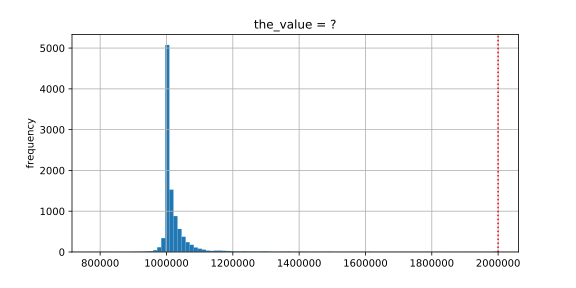
\includegraphics[width=1.1\textwidth]{../sync/parallel-add-histogram}
\end{frame}

\begin{frame}{but how?}
    \begin{itemize}
    \item probably not possible on single core
        \begin{itemize}
            \item exceptions can't occur in the middle of \texttt{add} instruction
        \end{itemize}
    \item \ldots but `add to memory' implemented with multiple steps
        \begin{itemize}
        \item still needs to load, add, store internally
        \item can be interleaved with what other cores do
        \end{itemize}
        \vspace{.5cm}
    \item<2-> {\small (and actually it's more complicated than that --- we'll talk later)}
    \end{itemize}
\end{frame}



\subsection{what is atomic?}

\begin{frame}{so, what is actually atomic}
    \begin{itemize}
    \item for now we'll assume: load/stores of `words' 
        \begin{itemize}
        \item  (64-bit machine = 64-bits words)
        \end{itemize}
        \vspace{.5cm}
    \item in general: \myemph{processor designer will tell you}
    \item their job to design caches, etc. to work as documented
    \end{itemize}
\end{frame}


\section{definitions: mutual exclusion, critical section}
\begin{frame}{some definitions}
\begin{itemize}
\item \textbf{mutual exclusion}: ensuring only one thread does a particular thing at a time
    \begin{itemize}
        \item like updating shared balance
    \end{itemize}
\item<2-> \textbf{critical section}: code that exactly one thread can execute at a time
    \begin{itemize}
        \item result of mutual exclusion
    \end{itemize}
\item<3-> \textbf{lock}: object only one thread can hold at a time
    \begin{itemize}
        \item interface for creating critical sections
    \end{itemize}
\end{itemize}
\end{frame}


\section{read-modify-write atomic operations}
\begin{frame}{atomic read-modfiy-write}
    \begin{itemize}
    \item really hard to build locks for atomic load store
        \begin{itemize}
        \item and normal load/stores aren't even atomic\ldots
        \end{itemize}
    \item \ldots so processors provide \myemph{read/modify/write} operations
        \vspace{.5cm}
    \item one instruction that\\\textit{atomically}\\reads \textit{and} modifies \textit{and} writes back a value
    \end{itemize}
\end{frame}

\subsection{x86 atomic exchange} 
\begin{frame}[fragile,label=atomicXchg]{x86 atomic exchange}
\begin{lstlisting}[language=myasm]
lock xchg (%ecx), %eax
\end{lstlisting}
\begin{itemize}
    \item atomic exchange
    \item \texttt{temp $\leftarrow$ M[ECX]}
    \item \texttt{M[ECX] $\leftarrow$ EAX}
    \item \texttt{EAX $\leftarrow$ temp}
    \item \ldots without being interrupted by other processors, etc.
\end{itemize}
\end{frame}


\begin{frame}{implementing atomic exchange}
    \begin{itemize}
    \item make sure other processors don't have cache block
    \item do read+modify+write operation
    \vspace{.5cm}
    \item recall: Modified state = ``I am the only one with a copy''
    \end{itemize}
\end{frame}



\section{locks}
\begin{frame}{lock analogy}
    \begin{itemize}
    \item agreement: whoever holds the flag can access shared resource
        \begin{itemize}
        \item flag doesn't actually do anything by itself\ldots
        \end{itemize}
    \item acquire/lock $\approx$ wait for and grab flag from table
    \item release/unlock $\approx$ put flag back on table
    \vspace{.5cm}
    \item<2-> agreement is \myemph{voluntary}
        \begin{itemize}
        \item thread tries to manipulate shared resource without lock? \\
            lock won't stop it\ldots
        \end{itemize}
    \item<2-> lock is \textit{held} by particular thread
    \end{itemize}
\end{frame}

% FIXME: lock analogy: hat
\begin{frame}[fragile,label=lockDefn]{the lock primitive}
    \begin{itemize}
    \item locks: an object with (at least) two operations:
        \begin{itemize}
        \item \textit{acquire} or \textit{lock} --- wait until lock is free, then ``grab'' it
        \item \textit{release} or \textit{unlock} --- let others use lock, wakeup waiters
        \end{itemize}
    \item typical usage: everyone acquires lock before using shared resource
        \begin{itemize}
        \item forget to acquire lock? weird things happen
        \end{itemize}
    \end{itemize}
\begin{lstlisting}[language=C++,style=small]
Lock(MilkLock);
if (no milk) {
    buy milk
}
Unlock(MilkLock);
\end{lstlisting}
\end{frame}

\begin{frame}[fragile,label=pthreadMutex]{pthread mutex}
\begin{lstlisting}[language=C++,style=small]
#include <pthread.h>

pthread_mutex_t MilkLock;
pthread_mutex_init(&MilkLock, NULL);
    // or: pthread_mutex_t MilkLock =
    //              PTHREAD_MUTEX_INITIALIZER;
...
pthread_mutex_lock(&MilkLock);
if (no milk) {
    buy milk
}
pthread_mutex_unlock(&MilkLock);
\end{lstlisting}
\end{frame}


\subsection{exercise}
\begin{frame}[fragile,label=lockEx]{exercise}
    \vspace{-0.5cm}
\begin{lstlisting}[style=smaller]
pthread_mutex_t lock1 = PTHREAD_MUTEX_INITIALIZER;
pthread_mutex_t lock2 = PTHREAD_MUTEX_INITIALIZER;
string one = "init one", two = "init two";
void ThreadA() {
    pthread_mutex_lock(&lock1);
    one = "one in ThreadA";  // (A1)
    pthread_mutex_unlock(&lock1);
    pthread_mutex_lock(&lock2);
    two = "two in ThreadA";  // (A2)
    pthread_mutex_unlock(&lock2);
}
void ThreadB() {
    pthread_mutex_lock(&lock1);
    one = "one in ThreadB";  // (B1)
    pthread_mutex_lock(&lock2);
    two = "two in ThreadB";  // (B2)
    pthread_mutex_unlock(&lock2);
    pthread_mutex_unlock(&lock1);
}
\end{lstlisting}
possible values of one/two after A+B run?
\end{frame}

\begin{frame}<0>[fragile,label=lockExSln]{solution}
\begin{itemize}
\item B1+A2
    \begin{itemize}
    \item A: L(1) A1 U(1) L
    \item B: L(1) B1 L(2) B2 U(2) U(1)
    \item A: L(2) A2 U(2)
    \end{itemize}
\item NOT A1+B2
    \begin{itemize}
    \item would need to run B1 before A1 before A2 before B2
    \item not possible because Lock1 held for entire B1+B2 operation
    \item so cannot fit A1+A2 in between B1 and B2
    \end{itemize}
\end{itemize}
\end{frame}

\iftoggle{heldback}{}{\againframe<1>{lockExSln}}

\begin{frame}[fragile,label=lockExAlt1]{exercise (alternate 1)}
    \vspace{-0.5cm}
\begin{lstlisting}[style=smaller]
pthread_mutex_t lock1 = PTHREAD_MUTEX_INITIALIZER;
pthread_mutex_t lock2 = PTHREAD_MUTEX_INITIALIZER;
string one = "init one", two = "init two";
void ThreadA() {
    pthread_mutex_lock(&lock2);
    two = "two in ThreadA";  // (A2)
    pthread_mutex_unlock(&lock2);
    pthread_mutex_lock(&lock1);
    one = "one in ThreadA";  // (A1)
    pthread_mutex_unlock(&lock1);
}
void ThreadB() {
    pthread_mutex_lock(&lock1);
    one = "one in ThreadB";  // (B1)
    pthread_mutex_lock(&lock2);
    two = "two in ThreadB";  // (B2)
    pthread_mutex_unlock(&lock2);
    pthread_mutex_unlock(&lock1);
}
\end{lstlisting}
possible values of one/two after A+B run?
\end{frame}

\begin{frame}[fragile,label=lockExAlt2]{exercise (alternate 2)}
    \vspace{-0.5cm}
\begin{lstlisting}[style=smaller]
pthread_mutex_t lock1 = PTHREAD_MUTEX_INITIALIZER;
pthread_mutex_t lock2 = PTHREAD_MUTEX_INITIALIZER;
string one = "init one", two = "init two";
void ThreadA() {
    pthread_mutex_lock(&lock2);
    two = "two in ThreadA";  // (A2)
    pthread_mutex_unlock(&lock2);
    pthread_mutex_lock(&lock1);
    one = "one in ThreadA";  // (A1)
    pthread_mutex_unlock(&lock1);
}
void ThreadB() {
    pthread_mutex_lock(&lock1);
    one = "one in ThreadB";  // (B1)
    pthread_mutex_unlock(&lock1);
    pthread_mutex_lock(&lock2);
    two = "two in ThreadB";  // (B2)
    pthread_mutex_unlock(&lock2);
}
\end{lstlisting}
possible values of one/two after A+B run?
\end{frame}


\subsection{pthread\_mutex: lock where you unlock}
\begin{frame}{POSIX mutex restrictions}
\begin{itemize}
\item pthread\_mutex rule: \myemph{unlock from same thread you lock in}
\vspace{.5cm}
\item implementation I gave before --- not a problem
\item \ldots but there other ways to implement mutexes
    \begin{itemize}
    \item e.g. might involve comparing with ``holding'' thread ID
    \end{itemize}
\end{itemize}
\end{frame}


\section{preview: beyond locks}
\begin{frame}{are locks enough?}
\begin{itemize}
    \item do we need more than locks?
\end{itemize}
\end{frame}

\begin{frame}{example 1: pipes?}
\begin{itemize}
\item suppose we want to implement a pipe with threads
\item \texttt{read} sometimes needs to wait for a \texttt{write}
\item don't want busy-wait
\begin{itemize}
\item (and trick of having writer unlock() so reader can finish a lock() is illegal)
\end{itemize}
\end{itemize}
\end{frame}

\begin{frame}{more synchronization primitives}
    \begin{itemize}
    \item need other ways to wait for threads to finish
    \item we'll introduce several synchronization ideas beyond locks:
        \begin{itemize}
        \item barriers --- (today)
        \item condition variables / monitors
        \item counting semaphores
        \item reader/writer locks
        \end{itemize}
    \end{itemize}
\end{frame}



\section{barriers}
\begin{frame}{barriers}
\begin{itemize}
\item compute minimum of 100M element array with 2 processors
\item algorithm:
\vspace{.5cm}
\item compute minimum of 50M of the elements on each CPU
    \begin{itemize}
    \item one thread for each CPU
    \end{itemize}
\item \myemph<2>{wait for all computations to finish}
\item take minimum of all the minimums
\end{itemize}
\end{frame}

\begin{frame}[fragile,label=barrierAPI]{barriers API}
\begin{itemize}
\item barrier.Initialize(NumberOfThreads)
\item barrier.Wait() --- return after all threads have waited
\vspace{.5cm}
\item idea: multiple threads perform computations in parallel
\item threads wait for \myemph{all other threads} to call Wait()
\end{itemize}
\end{frame}

\begin{frame}[fragile,label=barrierWait]{barrier: waiting for finish}
\begin{tikzpicture}
\node[label={north:Thread 0}] (code one) {
\begin{lstlisting}[language=C++,style=smaller]
partial_mins[0] = 
    /* min of first
       50M elems */;

barrier.Wait();


total_min = min(
    partial_mins[0],
    partial_mins[1]
);
\end{lstlisting}
};
\node[anchor=south] (code zero) at ([yshift=1cm]code one.north) {
\begin{lstlisting}[language=C++,style=smaller]
barrier.Initialize(2);
\end{lstlisting}
};

\node[label={north:Thread 1},anchor=north west] (code two) at ([xshift=1cm]code one.north east) {
\begin{lstlisting}[language=C++,style=smaller]


partial_mins[1] =
    /* min of last
       50M elems */
barrier.Wait();
\end{lstlisting}
};
\end{tikzpicture}
\end{frame}

\begin{frame}[fragile,label=barrierReuse]{barriers: reuse}
\begin{tikzpicture}
\node[label={north:Thread 0}] (code one) {
\begin{lstlisting}[
    language=C++,style=smaller,
    moredelim={**[is][\btHL<2|handout:0>]{@2}{2@}},
    moredelim={**[is][\btHL<3|handout:0>]{@3}{3@}},
    moredelim={**[is][\btHL<3|handout:0>]{@4}{4@}},
]
@2results[0][0]2@ = getInitial(0);
barrier.Wait();

@4results[1][0]4@ =
    computeFrom(0, 
        results[0][0],
        @3results[0][1]3@
    );
barrier.Wait();

results[2][0] =
    computeFrom(0,
        results[1][0],
        results[1][1]
    );
\end{lstlisting}
};
\node[label={north:Thread 1},anchor=north west] (code two) at ([xshift=1cm]code one.north east) {
\begin{lstlisting}[
    language=C++,style=smaller,
    moredelim={**[is][\btHL<2|handout:0>]{@2}{2@}},
    moredelim={**[is][\btHL<3|handout:0>]{@3}{3@}},
    moredelim={**[is][\btHL<3|handout:0>]{@4}{4@}},
]
@3results[0][1]3@ = getInitial(1);
barrier.Wait();

results[1][1] =
    computeFrom(1, 
        @2results[0][0],2@
        results[0][1]
    );
barrier.Wait();

results[2][1] =
    computeFrom(1,
        @4results[1][0]4@,
        results[1][1]
    );
\end{lstlisting}
};
\end{tikzpicture}
\end{frame}

\begin{frame}[fragile,label=pthreadBarrier]{pthread barriers}
\begin{lstlisting}[language=C++,style=smaller]
pthread_barrier_t barrier;
pthread_barrier_init(
    &barrier,
    NULL /* attributes */,
    numberOfThreads
);
...
...
pthread_barrier_wait(&barrier);
\end{lstlisting}
\end{frame}



\section{life HW}
\begin{frame}[fragile,label=lifeHW]{life homework (pseudocode)}
\begin{lstlisting}[
    language=C++,style=smaller,
    moredelim={**[is][\btHL<2|handout:0>]{@2}{2@}},
    moredelim={**[is][\btHL<3|handout:0>]{@3}{3@}},
    moredelim={**[is][\btHL<3|handout:0>]{@4}{4@}},
]
for (int time = 0; time < MAX_ITERATIONS; ++time) {
    for (int y = 0; y < size; ++y) {
        for (int x = 0; x < size; ++x) {
            to_grid(x, y) = computeValue(from_grid, x, y);
        }
    }
    swap(from_grid, to_grid);
}
\end{lstlisting}
\end{frame}

\begin{frame}{life homework}
\begin{itemize}
\item compute grid of values for time $t$ from grid for time $t-1$
    \begin{itemize}
    \item compute new value at $i,j$ based on surrounding values
    \end{itemize}
\vspace{.5cm}
\item parallel version: produce parts of grid in different threads
\item use barriers to finish time $t$ before going to time $t+1$
\end{itemize}
\end{frame}




\section{aside: reordering}

\section{revisiting atomicity}
\subsection{compiler reordering}
\begin{frame}[fragile,label=compReorder]{compilers move loads/stores (1)}
\begin{lstlisting}[language=C++,style=small,
    moredelim={**[is][\btHL<2|handout:2>]{@2}{2@}},
    moredelim={**[is][\btHL<3|handout:3>]{@3}{3@}},
    moredelim={**[is][\btHL<4|handout:4>]{@4}{4@}},
    moredelim={**[is][\btHL<5|handout:5>]{@5}{5@}},
]
void Alice() {
    note_from_alice = 1;
    @2do {} while (note_from_bob);2@
    if (no_milk) {++milk;}
}
\end{lstlisting}
\hrule
\begin{lstlisting}[language=myasm,style=smaller,
    moredelim={**[is][\btHL<2|handout:2>]{@2}{2@}},
    moredelim={**[is][\btHL<3|handout:3>]{@3}{3@}},
    moredelim={**[is][\btHL<4|handout:4>]{@4}{4@}},
    moredelim={**[is][\btHL<5|handout:5>]{@5}{5@}},
]
Alice:
  movl $1, note_from_alice  // note_from_alice <- 1
  movl note_from_bob, %eax  // eax <- note_from_bob
.L2:
  @2testl %eax, %eax2@
  @2jne .L22@                   // while (eax == 0) repeat
  cmpl $0, no_milk          // if (no_milk != 0) ...
  ...
\end{lstlisting}
\end{frame}

\begin{frame}[fragile,label=compReorder2]{compilers move loads/stores too (2)}
\begin{lstlisting}[language=C++,style=smaller,
    moredelim={**[is][\btHL<2|handout:2>]{@2}{2@}},
    moredelim={**[is][\btHL<3|handout:3>]{@3}{3@}},
    moredelim={**[is][\btHL<4|handout:4>]{@4}{4@}},
    moredelim={**[is][\btHL<5|handout:5>]{@5}{5@}},
]
void Alice() {
    @3note_from_alice = 1;3@  // "Alice waiting" signal for Bob()
    do {} while (note_from_bob);
    if (no_milk) {++milk;}
    @2note_from_alice = 2;2@
}
\end{lstlisting}
\hrule
\begin{lstlisting}[language=myasm,style=smaller,
    moredelim={**[is][\btHL<2|handout:2>]{@2}{2@}},
    moredelim={**[is][\btHL<3|handout:3>]{@3}{3@}},
    moredelim={**[is][\btHL<4|handout:4>]{@4}{4@}},
    moredelim={**[is][\btHL<5|handout:5>]{@5}{5@}},
]
Alice:  
  // compiler optimization: don't set note_from_alice to 1,
  // (why? it will be set to 2 anyway)
  @3movl note_from_bob, %eax3@  // eax <- note_from_bob
.L2:
  testl %eax, %eax          
  jne .L2                   // while (eax == 0) repeat
  ...
  @2movl $2, note_from_alice2@  // note_from_alice <- 2
\end{lstlisting}
\end{frame}


\subsection{processor reordering}
\begin{frame}[fragile,label=loadReorderSetup]{a simple race}
\begin{minipage}{0.45\textwidth}
\begin{lstlisting}[language=myasm,style=smaller]
thread_A:
    movl $1, x   /* x <- 1 */
    movl y, %eax /* return y */
    ret
\end{lstlisting}
\end{minipage}
\begin{minipage}{0.45\textwidth}
\begin{lstlisting}[language=myasm,style=smaller]
thread_B:
    movl $1, y   /* y <- 1 */
    movl x, %eax /* return x */
    ret
\end{lstlisting}
\end{minipage}
\\
\begin{lstlisting}[language=C++,style=smaller]
x = y = 0;
pthread_create(&A, NULL, thread_A, NULL);
pthread_create(&B, NULL, thread_B, NULL);
pthread_join(A, &A_result); pthread_join(B, &B_result);
printf("A:%d B:%d\n", (int) A_result, (int) B_result);
\end{lstlisting}
\begin{itemize}
\item<2-> if loads/stores atomic, then possible results:
    \begin{itemize}
    \item A:1 B:1 --- both moves into x and y, then both moves into eax execute
    \item A:0 B:1 --- thread A executes before thread B
    \item A:1 B:0 --- thread B executes before thread A
    \end{itemize}
\end{itemize}
\end{frame}

\begin{frame}[fragile,label=loadReorderExpResults]{a simple race: results}
\begin{minipage}{0.45\textwidth}
\begin{lstlisting}[language=myasm,style=smaller]
thread_A:
    movl $1, x   /* x <- 1 */
    movl y, %eax /* return y */
    ret
\end{lstlisting}
\end{minipage}
\begin{minipage}{0.45\textwidth}
\begin{lstlisting}[language=myasm,style=smaller]
thread_B:
    movl $1, y   /* y <- 1 */
    movl x, %eax /* return x */
    ret
\end{lstlisting}
\end{minipage}
\begin{lstlisting}[language=C++,style=smaller]
x = y = 0;
pthread_create(&A, NULL, thread_A, NULL);
pthread_create(&B, NULL, thread_B, NULL);
pthread_join(A, &A_result); pthread_join(B, &B_result);
printf("A:%d B:%d\n", (int) A_result, (int) B_result);
\end{lstlisting}
\vspace{-.5cm}
\begin{center}
\small my desktop, 100M trials: \\
\begin{tabular}{r|l|l}
frequency & result & ~ \\ \hline
$99\,823\,739$ & A:0 B:1 & (`A executes before B') \\
$171\,161$& A:1 B:0 & (`B executes before A') \\
$4\,706$ & A:1 B:1 & (`execute moves into x+y first') \\
\myemph<2>{$394$} & \myemph<2>{A:0 B:0} & \myemph<2>{???} \\
\end{tabular}
\end{center}
\end{frame}


\subsection{why reorder?}

\begin{frame}[fragile]{why reorder here?}
\begin{tikzpicture}
\node (thread A code) {
\begin{lstlisting}[language=myasm,style=smaller]
thread_A:
    movl $1, x   /* x <- 1 */
    movl y, %eax /* return y */
    ret
\end{lstlisting}
};
\node[anchor=north west] (thread B code) at ([xshift=.5cm]thread A code.north east) {
\begin{lstlisting}[language=myasm,style=smaller]
thread_B:
    movl $1, y   /* y <- 1 */
    movl x, %eax /* return x */
    ret
\end{lstlisting}
};
\end{tikzpicture}
\begin{itemize}
\item thread A: faster to load \texttt{y} right now!
\item \ldots rather than wait for write of \texttt{x} to finish
\end{itemize}
\end{frame}


\usetikzlibrary{calc}

\begin{frame}{why load/store reordering?}
\begin{itemize}
\item fast processor designs can execute instructions out of order
\item goal: do something instead of waiting for slow memory accesses, etc.
\item more on this later in the semester
\end{itemize}
\end{frame}





\section{pthreads and load/store reordering}
\begin{frame}{pthreads and reordering}
    \begin{itemize}
    \item many pthreads functions \myemph{prevent reordering}
        \begin{itemize}
        \item everything before function call actually happens before 
        \end{itemize}
    \item includes \myemph{preventing some optimizations}
        \begin{itemize}
        \item e.g. keeping global variable in register for too long
        \end{itemize}
    \vspace{.5cm}
    \item pthread\_mutex\_lock/unlock, pthread\_create, pthread\_join, \ldots
        \begin{itemize}
        \item basically: if pthreads is waiting for/starting something, no weird ordering
        \end{itemize}
    \item implementation part 1: prevent compiler reordering
    \item implementation part 2: use special instructions
        \begin{itemize}
        \item example: x86 \texttt{mfence} instruction
        \end{itemize}
    \end{itemize}
\end{frame}







\section{barriers}
\begin{frame}{barriers}
\begin{itemize}
\item compute minimum of 100M element array with 2 processors
\item algorithm:
\vspace{.5cm}
\item compute minimum of 50M of the elements on each CPU
    \begin{itemize}
    \item one thread for each CPU
    \end{itemize}
\item \myemph<2>{wait for all computations to finish}
\item take minimum of all the minimums
\end{itemize}
\end{frame}

\begin{frame}[fragile,label=barrierAPI]{barriers API}
\begin{itemize}
\item barrier.Initialize(NumberOfThreads)
\item barrier.Wait() --- return after all threads have waited
\vspace{.5cm}
\item idea: multiple threads perform computations in parallel
\item threads wait for \myemph{all other threads} to call Wait()
\end{itemize}
\end{frame}

\begin{frame}[fragile,label=barrierWait]{barrier: waiting for finish}
\begin{tikzpicture}
\node[label={north:Thread 0}] (code one) {
\begin{lstlisting}[language=C++,style=smaller]
partial_mins[0] = 
    /* min of first
       50M elems */;

barrier.Wait();


total_min = min(
    partial_mins[0],
    partial_mins[1]
);
\end{lstlisting}
};
\node[anchor=south] (code zero) at ([yshift=1cm]code one.north) {
\begin{lstlisting}[language=C++,style=smaller]
barrier.Initialize(2);
\end{lstlisting}
};

\node[label={north:Thread 1},anchor=north west] (code two) at ([xshift=1cm]code one.north east) {
\begin{lstlisting}[language=C++,style=smaller]


partial_mins[1] =
    /* min of last
       50M elems */
barrier.Wait();
\end{lstlisting}
};
\end{tikzpicture}
\end{frame}

\begin{frame}[fragile,label=barrierReuse]{barriers: reuse}
\begin{tikzpicture}
\node[label={north:Thread 0}] (code one) {
\begin{lstlisting}[
    language=C++,style=smaller,
    moredelim={**[is][\btHL<2|handout:0>]{@2}{2@}},
    moredelim={**[is][\btHL<3|handout:0>]{@3}{3@}},
    moredelim={**[is][\btHL<3|handout:0>]{@4}{4@}},
]
@2results[0][0]2@ = getInitial(0);
barrier.Wait();

@4results[1][0]4@ =
    computeFrom(0, 
        results[0][0],
        @3results[0][1]3@
    );
barrier.Wait();

results[2][0] =
    computeFrom(0,
        results[1][0],
        results[1][1]
    );
\end{lstlisting}
};
\node[label={north:Thread 1},anchor=north west] (code two) at ([xshift=1cm]code one.north east) {
\begin{lstlisting}[
    language=C++,style=smaller,
    moredelim={**[is][\btHL<2|handout:0>]{@2}{2@}},
    moredelim={**[is][\btHL<3|handout:0>]{@3}{3@}},
    moredelim={**[is][\btHL<3|handout:0>]{@4}{4@}},
]
@3results[0][1]3@ = getInitial(1);
barrier.Wait();

results[1][1] =
    computeFrom(1, 
        @2results[0][0],2@
        results[0][1]
    );
barrier.Wait();

results[2][1] =
    computeFrom(1,
        @4results[1][0]4@,
        results[1][1]
    );
\end{lstlisting}
};
\end{tikzpicture}
\end{frame}

\begin{frame}[fragile,label=pthreadBarrier]{pthread barriers}
\begin{lstlisting}[language=C++,style=smaller]
pthread_barrier_t barrier;
pthread_barrier_init(
    &barrier,
    NULL /* attributes */,
    numberOfThreads
);
...
...
pthread_barrier_wait(&barrier);
\end{lstlisting}
\end{frame}



\subsection{exercise}
\begin{frame}[fragile]{exercise}
\lstset{language=C,style=smaller}
\begin{lstlisting}
pthread_barrier_t barrier;
int x = 0, y = 0;
void thread_one() {
    y = 10;
    pthread_barrier_wait(&barrier);
    y = x + y;
    pthread_barrier_wait(&barrier);
    pthread_barrier_wait(&barrier);
    printf("%d %d\n", x, y);
}

void thread_two() {
    x = 20;
    pthread_barrier_wait(&barrier);
    pthread_barrier_wait(&barrier);
    x = x + y;
    pthread_barrier_wait(&barrier);
}
\end{lstlisting}
\begin{itemize}
\item if both thread\_one, thread\_two run at once
\item output? 
\end{itemize}
\end{frame}


\section{life HW}
\begin{frame}[fragile,label=lifeHW]{life homework (pseudocode)}
\begin{lstlisting}[
    language=C++,style=smaller,
    moredelim={**[is][\btHL<2|handout:0>]{@2}{2@}},
    moredelim={**[is][\btHL<3|handout:0>]{@3}{3@}},
    moredelim={**[is][\btHL<3|handout:0>]{@4}{4@}},
]
for (int time = 0; time < MAX_ITERATIONS; ++time) {
    for (int y = 0; y < size; ++y) {
        for (int x = 0; x < size; ++x) {
            to_grid(x, y) = computeValue(from_grid, x, y);
        }
    }
    swap(from_grid, to_grid);
}
\end{lstlisting}
\end{frame}

\begin{frame}{life homework}
\begin{itemize}
\item compute grid of values for time $t$ from grid for time $t-1$
    \begin{itemize}
    \item compute new value at $i,j$ based on surrounding values
    \end{itemize}
\vspace{.5cm}
\item parallel version: produce parts of grid in different threads
\item use barriers to finish time $t$ before going to time $t+1$
\end{itemize}
\end{frame}




\section{producer/consumer problem}
\usetikzlibrary{arrows.meta,shapes.multipart}

\begin{frame}{example: producer/consumer}
\begin{tikzpicture}
    \node[minimum width=3cm,minimum height=1cm,draw,very thick,fill=blue!20] (producer) {producer};
    \node[minimum height=0.75cm,draw,very thick,fill=violet!20,
          anchor=west,rectangle split,rectangle split horizontal,
          rectangle split parts=4] (buffer) at ([xshift=1.5cm]producer.east) {buffer
            \hspace{3cm}};
    \node[minimum width=3cm,minimum height=1cm,draw,very thick,fill=blue!20,
          anchor=west] (consumer) at ([xshift=1.5cm]buffer.east) {consumer};

    \begin{scope}[very thick,>=Latex]
        \draw[->] (producer)  -- (buffer);
        \draw[->] (buffer)  -- (consumer);
    \end{scope}
\end{tikzpicture}
    \begin{itemize}
        \item shared buffer (queue) of fixed size
            \begin{itemize}
            \item one or more producers inserts into queue
            \item one or more consumers removes from queue
            \end{itemize}
        \item<2-> producer(s) and consumer(s) don't work in lockstep
            \begin{itemize}
            \item (might need to wait for each other to catch up)
            \end{itemize}
        \item<3-> example: C compiler
            \begin{itemize}
            \item preprocessor $\rightarrow$ compiler $\rightarrow$ assembler $\rightarrow$ linker
            \end{itemize}
    \end{itemize}
\end{frame}




\section{monitors}

\subsection{introduction}
\usetikzlibrary{arrows.meta,calc,chains,fit,matrix}

\begin{frame}{monitors/condition variables}
\begin{itemize}
\item \myemph{locks} for mutual exclusion
\item \myemph{condition variables} for waiting for event
    \begin{itemize}
    \item operations: wait (for event); signal/broadcast (that event happened)
    \end{itemize}
\item related data structures
\vspace{.5cm}
\item \myemph{monitor} = lock + 0 or more condition variables + shared data
    \begin{itemize}
    \item Java: every object is a monitor (has instance variables, built-in lock, cond. var)
    \item pthreads: build your own: provides you locks + condition variables
    \end{itemize}
\end{itemize}
\end{frame}

\begin{frame}[fragile,label=monitorIdea]{monitor idea}
\begin{tikzpicture}
\tikzset{
    hilite red on/.style={alt=<#1>{fill=red!10}},
    hilite blue on/.style={alt=<#1>{fill=blue!10}},
    >=Latex,
    queue node/.style={draw,thick,minimum width=.6cm,minimum height=.6cm},
    queue connect/.style={draw,->,ultra thick},
}
\matrix[
    tight matrix,
    nodes={draw,thick,text width=4cm,font=\small},
    label={[font=\small]north:a monitor},
    ] (monitor) {
    |[hilite red on={2-}]| lock \\
    shared data \\
    |[hilite blue on={4-}]| condvar 1 \\
    |[hilite blue on={4-}]| condvar 2 \\
    \ldots \\
    |[minimum height=0.2mm]| {} \\
    operation1(\ldots)\\
    operation2(\ldots) \\
};
\begin{visibleenv}<2-3|handout:2>
    \node[draw=red,ultra thick,inner sep=0mm,fit=(monitor-2-1) (monitor-5-1)] {};
\end{visibleenv}
\begin{visibleenv}<2|handout:0>
    \node[red,anchor=north west,align=left] at (monitor-1-1.north east) {
            lock must be acquired \\
            before accessing \\
            any part of monitor's stuff
    };
\end{visibleenv}
\begin{visibleenv}<3->
    \begin{scope}[
        start chain=going right,
        every join/.style={queue connect},
        every node/.style={queue node,on chain,join,fill=red!10},
    ]
    \node[anchor=west] (lock queue 1) at ([xshift=1cm]monitor-1-1.east) {};
    \node (lock queue 2) {};
    \node (lock queue 3) {};
    \end{scope}
    \draw[->,dashed,ultra thick] (monitor-1-1) -- (lock queue 1);
\end{visibleenv}
\begin{visibleenv}<3->
    \node[anchor=west,align=left,text=red!20!black] at ([xshift=0cm]lock queue 3.east) {
        threads waiting for lock
    };
\end{visibleenv}
\begin{visibleenv}<4->
    \begin{scope}[
        start chain=going right,
        every join/.style={queue connect},
        every node/.style={queue node,on chain,join,fill=blue!10},
    ]
    \node[anchor=west] (condvar 1 queue 1) at ([xshift=1cm,yshift=-1cm]monitor-3-1.east) {};
    \node (condvar 1 queue 2) {};
    \node (condvar 1 queue 3) {};
    \end{scope}
    \draw[->,dashed,ultra thick] (monitor-3-1.east) -- (condvar 1 queue 1);

    \begin{scope}[
        start chain=going right,
        every join/.style={queue connect},
        every node/.style={queue node,on chain,join,fill=blue!10},
    ]
    \node[anchor=west] (condvar 2 queue 1) at ([xshift=1cm,yshift=-1.5cm]monitor-4-1.east) {};
    \node (condvar 2 queue 2) {};
    \node (condvar 2 queue 3) {};
    \end{scope}
    \draw[->,dashed,ultra thick] (monitor-4-1.east) -- (condvar 2 queue 1);
    \node[anchor=west,align=left,text=blue!20!black] at ($(condvar 2 queue 3.north east)!0.5!(condvar 1 queue 3.south east)$) {
        threads waiting for \\
        condition to be true \\ 
        about shared data
    };
\end{visibleenv}
\end{tikzpicture}
\end{frame}

\begin{frame}[fragile,label=condVarOps]{condvar operations}
\begin{tikzpicture}
\tikzset{
    hilite red on/.style={alt=<#1>{fill=red!10}},
    hilite blue on/.style={alt=<#1>{fill=blue!10}},
    >=Latex,
    queue node/.style={draw,thick,minimum width=.6cm,minimum height=.6cm},
    queue connect/.style={draw,->,ultra thick},
}
\matrix[
    tight matrix,
    nodes={draw,thick,text width=4cm,font=\small},
    label={[font=\small]north:a monitor},
    ] (monitor) {
    |[hilite red on={1-}]| lock \\
    shared data \\
    |[hilite blue on={1-}]| condvar 1 \\
    |[hilite blue on={1-}]| condvar 2 \\
    \ldots \\
    |[minimum height=0.2mm]| {} \\
    operation1(\ldots)\\
    operation2(\ldots) \\
};
    %\node[draw=red,ultra thick,inner sep=0mm,fit=(monitor-2-1) (monitor-5-1)] {};
    \begin{scope}[
        start chain=going right,
        %every join/.style={queue connect},
        every node/.style={queue node,on chain,fill=red!10},
    ]
    \node[anchor=west,alt=<3>{opacity=0.2}] (lock queue 1) at ([xshift=1cm]monitor-1-1.east) {};
    \node (lock queue 2) {};
    \node (lock queue 3) {};
    \end{scope}
    \draw[queue connect,alt=<3>{opacity=0.2}] (lock queue 1) --(lock queue 2);
    \draw[queue connect] (lock queue 2) --(lock queue 3);
    \draw[->,dashed,ultra thick,alt=<3>{opacity=0}] (monitor-1-1) -- (lock queue 1);
    \begin{visibleenv}<3>
        \draw[->,dashed,ultra thick,red,out=-15,in=-155] (monitor-1-1.east) to (lock queue 2);
    \end{visibleenv}
    \node[anchor=west,align=left,text=red!20!black] at ([xshift=0cm]lock queue 3.east) {
        threads waiting for lock
    };
    \begin{scope}[
        start chain=going right,
        every join/.style={queue connect,alt={<4,5>{opacity=0.2}}},
        every node/.style={queue node,on chain,join,fill=blue!10,alt=<4>{draw=red,dashed,thick}},
    ]
    \node[anchor=west] (condvar 1 queue 1) at ([xshift=1cm,yshift=-1cm]monitor-3-1.east) {};
    \node[alt=<5>{draw=red,dashed,thick}] (condvar 1 queue 2) {};
    \node (condvar 1 queue 3) {};
    \end{scope}
    \draw[->,dashed,ultra thick,alt=<4>{opacity=0.2}] (monitor-3-1.east) -- (condvar 1 queue 1);
    \begin{visibleenv}<5>
        \draw[->,dashed,ultra thick,red,in=-155,out=-20] (condvar 1 queue 1) to (condvar 1 queue 3);
    \end{visibleenv}

    \begin{scope}[
        start chain=going right,
        every join/.style={queue connect},
        every node/.style={queue node,on chain,join,fill=blue!10},
    ]
    \node[anchor=west] (condvar 2 queue 1) at ([xshift=1cm,yshift=-1.5cm]monitor-4-1.east) {};
    \node (condvar 2 queue 2) {};
    \node (condvar 2 queue 3) {};
    \end{scope}
    \draw[->,dashed,ultra thick] (monitor-4-1.east) -- (condvar 2 queue 1);
    \node[anchor=west,align=left,text=blue!20!black] at ($(condvar 2 queue 3.north east)!0.5!(condvar 1 queue 3.south east)$) {
        threads waiting for \\
        condition to be true \\ 
        about shared data
    };
    \node[anchor=south west,align=left] (oplist)  at ([yshift=.5cm,xshift=-3.5cm]monitor.north east) {
        \textcolor{blue!80!black}{condvar} operations: \\
        \myemph<2-3>{\textbf<2>{Wait(cv, lock)}} --- \myemph<3>{unlock} lock, \myemph<2>{add current thread} to cv queue \\
        \ldots and \myemph<3>{reacquire} lock before returning \\
        \myemph<4>{\textbf<4>{Broadcast(cv)}} --- remove all from condvar queue \\
        \myemph<5>{\textbf<5>{Signal(cv)}} --- remove one from condvar queue \\
    };
    \tikzset{
        queue change/.style={dashed,ultra thick,red},
    }
    \begin{visibleenv}<3>
        \draw[->,queue change,in=180,out=90] (lock queue 1.north) to ++(1cm,1cm)
            node[right,red,font=\small] {unlock lock --- allow thread from queue to go};
    \end{visibleenv}
    \begin{visibleenv}<2>
        \draw[->,queue change,in=180,out=90] (condvar 1 queue 3.north) to ++(1cm,1cm) node[right,queue node,draw=red,
            label={[font=\small]east:calling thread starts waiting}] {};
    \end{visibleenv}
    \begin{visibleenv}<3>
        \draw[->,black!50,in=180,out=90] (condvar 1 queue 3.north) to ++(1cm,1cm) node[right,queue node,draw=red,
            ] {};
    \end{visibleenv}
    \begin{visibleenv}<4>
        \coordinate (unqueue dest) at (lock queue 3.south);
        \draw[<-,queue change,in=-90,out=90] (condvar 1 queue 1.north) to (unqueue dest);
        \draw[<-,queue change,in=90,out=90] (condvar 1 queue 2.north) to (condvar 1 queue 1.north);
        \draw[<-,queue change,in=90,out=90] (condvar 1 queue 3.north) to (condvar 1 queue 2.north);
        \node[anchor=north west,text=red,font=\small,align=left] at (unqueue dest) {
            all threads removed from cv queue \\
            to start waiting for lock
        };
    \end{visibleenv}
    \begin{visibleenv}<5>
        \coordinate (unqueue dest) at (lock queue 3.south);
        \draw[<-,queue change,in=-90,out=90] (condvar 1 queue 2.north) to (unqueue dest);
        \node[anchor=north west,text=red,font=\small,align=left] at (unqueue dest) {
            any one thread removed from cv queue \\
            to start waiting for lock
        };
    \end{visibleenv}
\end{tikzpicture}
\end{frame}
  % FIXME: incomplete

\subsection{example: WaitForFinished}
\begin{frame}[fragile,label=finishedExample]{pthread cv usage}
\begin{lstlisting}[
    language=C++,style=size105,
    morekeywords={pthread_mutex_t,pthread_cond_t},
    moredelim={**[is][\btHL<2|handout:2>]{@2}{2@}}, 
    moredelim={**[is][\btHL<3|handout:3>]{@3}{3@}}, 
    moredelim={**[is][\btHL<4|handout:4>]{@4}{4@}}, 
    moredelim={**[is][\btHL<5|handout:5>]{@5}{5@}}, 
    escapeinside=QQ,
]
// MISSING: init calls, etc.
pthread_mutex_t lock;
bool finished;   // data, only accessed with after acquiring lock
pthread_cond_t finished_cv;  // to wait for 'finished' to be true

void WaitForFinished() {
  @2pthread_mutex_lock(&lock);2@Q\tikzmark{lock for wait}Q
  @3while (!finished) {3@Q\tikzmark{finished loop}Q
    @4pthread_cond_wait(&finished_cv, &lock);4@Q\tikzmark{wait}Q
  }
  pthread_mutex_unlock(&lock);
}

void Finish() {
  @2pthread_mutex_lock(&lock);2@Q\tikzmark{lock for finish}Q
  finished = true;
  @5pthread_cond_broadcast(&finished_cv);5@Q\tikzmark{broadcast}Q
  pthread_mutex_unlock(&lock);
}
\end{lstlisting}
\begin{tikzpicture}[overlay,remember picture]
\tikzset{
    >=Latex,
    explain box/.style={draw=red,text=black,very thick,align=left},
    point line/.style={very thick,red},
}

\begin{visibleenv}<2>
    \node[explain box,anchor=east,fill=white] (acquire text) at ([yshift=-1cm,xshift=-.5cm]current page.east) {
        acquire lock before \\ reading or writing \texttt{finished}
    };
    \draw[point line,<-] ([yshift=1.5mm]pic cs:lock for wait) -- (acquire text);
    \draw[point line,<-] ([yshift=1.5mm]pic cs:lock for finish) -- (acquire text);
\end{visibleenv}
\begin{visibleenv}<3>
    \node[explain box,anchor=east,fill=white,fill opacity=0.9] (loop text) at ([xshift=-.5cm]current page.east |- {pic cs:finished loop}) {
        check whether we need to wait at all \\
        {\small (why a loop? we'll explain later)}
    };
    \draw[point line,<-] ([yshift=1.5mm]pic cs:finished loop) -- (loop text);
\end{visibleenv}
\begin{visibleenv}<4>
    \node[explain box,anchor=east,fill=white,fill opacity=0.9] (wait text) at ([xshift=-.5cm,yshift=-2cm]current page.east) {
        know we need to wait  \\
        (finished can't change while we have lock) \\
        so wait, releasing lock\ldots
    };
    \draw[point line,<-] ([yshift=1.5mm]pic cs:wait) -- (wait text);
\end{visibleenv}
\begin{visibleenv}<5>
    \node[explain box,anchor=east,fill=white,fill opacity=0.9] (broadcast text) at ([yshift=2cm,xshift=-.5cm]current page.east |- {pic cs:broadcast}) {
        allow all waiters to proceed \\
        (once we unlock the lock)
    };
    \draw[point line,<-] ([yshift=1.5mm]pic cs:broadcast) -- (broadcast text);
\end{visibleenv}
\end{tikzpicture}
\end{frame}

\begin{frame}[fragile,label=waitForFinishTimeline1]{WaitForFinish timeline 1}
\lstset{language=C++,style=smaller}
\small
  \vspace{-.25cm}
\begin{tabular}{l|l}
  \textbf{WaitForFinish thread} & \textbf{Finish thread} \\ \hline\hline
\lstinline|mutex_lock(&lock)| & \\
(thread has lock)             & \\ \hline
~                             & \lstinline|mutex_lock(&lock)|  \\
~                             & (start waiting for lock)\\ \hline
\lstinline|while (!finished) ...| & \\
\lstinline|cond_wait(&finished_cv, &lock);| & \\
(start waiting for cv) & (done waiting for lock) \\ \hline
~ & \lstinline|finished = true| \\
~ & \lstinline|cond_broadcast(&finished_cv)| \\ \hline
(done waiting for cv) & ~ \\
(start waiting for lock) & ~ \\ \hline
~ & \lstinline|mutex_unlock(&lock)| \\ \hline
(done waiting for lock) \\
\lstinline|while (!finished) ...| & \\
(finished now true, so return) \\
\lstinline|mutex_unlock(&lock)| \\
\end{tabular}
\end{frame}

\begin{frame}[fragile,label=waitForFinishTimeline2]{WaitForFinish timeline 2}
\lstset{language=C++,style=smaller}
\small
  \vspace{-.25cm}
\begin{tabular}{l|l}
  \textbf{WaitForFinish thread} & \textbf{Finish thread} \\ \hline\hline
~                             & \lstinline|mutex_lock(&lock)|  \\
~                             & \lstinline|finished = true| \\ 
~                             & \lstinline|cond_broadcast(&finished_cv)| \\ 
~                             & \lstinline|mutex_unlock(&lock)| \\ \hline
\lstinline|mutex_lock(&lock)| & \\
\lstinline|while (!finished) ...| & \\
(finished now true, so return) \\
\lstinline|mutex_unlock(&lock)| \\
\end{tabular}
\end{frame}

\begin{frame}[fragile,label=whyLoop]{why the loop}
\begin{lstlisting}[language=C++,style=small]
while (!finished) {
  pthread_cond_wait(&finished_cv, &lock);
}
\end{lstlisting}
\begin{itemize}
  \item we only \texttt{broadcast} if \texttt{finished} is true
  \item so why check \texttt{finished} afterwards?
    \vspace{.5cm}

  \item<2-> pthread\_cond\_wait manual page: 
        \begin{itemize}
          \item ``\myemph{Spurious wakeups} ... may occur.''
            \end{itemize}
  \item<2-> spurious wakeup = \texttt{wait} returns even though nothing happened
\end{itemize}
\end{frame}



\subsection{unbounded queue with monitors}
\usetikzlibrary{arrows.meta,fit,matrix}

\begin{frame}[fragile,label=unboundedPC]{unbounded buffer producer/consumer}
\begin{lstlisting}[
    language=C++,
    basicstyle=\tt\fontsize{10}{11}\selectfont,
    morekeywords=pthread_mutex_t,
    morekeywords=pthread_cond_t,
    morekeywords=UnboundedQueue,
    moredelim={**[is][\btHL<2|handout:2>]{@2}{2@}},
    moredelim={**[is][\btHL<3|handout:3>]{@3}{3@}},
    moredelim={**[is][\btHL<4|handout:4>]{@4}{4@}},
    moredelim={**[is][\btHL<5-,3|handout:5-,3>]{@5}{5@}},
    escapeinside=XX,
]
pthread_mutex_t lock;
pthread_cond_t data_ready;
UnboundedQueue buffer;

Produce(item) {
    @2pthread_mutex_lock(&lock);2@
    buffer.enqueue(item);
    @4pthread_cond_signal(&data_ready);4@X\tikzmark{signal}X
    @2pthread_mutex_unlock(&lock);2@
}
Consume() {
    @2pthread_mutex_lock(&lock);2@
    while (@5buffer.empty()5@) {X\tikzmark{empty}X
        pthread_cond_wait(&data_ready, &lock);
    }X\tikzmark{after loop}X
    item = @3buffer.dequeue()3@;
    @2pthread_mutex_unlock(&lock);2@
    return item;
}
\end{lstlisting}
\begin{tikzpicture}[overlay,remember picture]
    \coordinate (place) at ([xshift=-.5cm,yshift=-1.5cm]current page.north east);
    \coordinate (place lower) at ([xshift=-.5cm,yshift=-4.25cm]current page.north east);
    \tikzset{
        box base/.style={draw=red,ultra thick,align=left,anchor=north east,fill=white},
        box/.style={box base,at={(place)}},
        box lower/.style={box base,at={(place lower)}},
        >=Latex,
    }
    \begin{visibleenv}<2>
        \node [box] {
            rule: never touch \texttt{buffer} \\
            without acquiring lock \\
            ~ \\
            otherwise: what if two threads \\ simultaneously en/dequeue?  \\
            {\small (both use same array/linked list entry?)} \\
            {\small (both reallocate array?)}
        };
    \end{visibleenv}
    \begin{visibleenv}<3>
        \node [box lower] {
            check if not empty \\
            if so, dequeue \\
            ~ \\
            okay because have lock
        };
        \draw[<-,very thick,draw=red] (pic cs:after loop) -- ++(6cm,0cm) node[right,align=left] {
            other threads can\textbf{not} dequeue here
        };
    \end{visibleenv}
    \begin{visibleenv}<4>
        \draw[<-,very thick,draw=red] ([yshift=1.5mm]pic cs:signal) -- ++(2cm,0cm) node[right,align=left] {
            wake one Consume thread \\ \textit{if any are waiting} \\
        };
    \end{visibleenv}
    \begin{visibleenv}<5->
        \draw[<-,very thick,draw=red] ([yshift=1.5mm]pic cs:empty) -- ++(1cm,-2cm)
        node[fill=white,draw=red,right,align=left,font=\fontsize{10.5}{10}\selectfont,inner sep=0.1mm] {
            \myemph<5>{0 iterations}: Produce() called before Consume() \\
            \myemph<6>{1 iteration}: Produce() signalled, probably \\
            \myemph<7-8>{2+ iterations}: spurious wakeup or \ldots?
        };
        \tikzset{
            timeline/.style={
                tight matrix,fill=white,
                nodes={text width=3.5cm,font=\fontsize{10.5}{11}\selectfont,fill=white,text depth=0.075cm,text height=0.25cm},
                at={([xshift=-0.75cm,yshift=-1.15cm]current page.north east)},
                anchor=north east,
                row 1/.style={nodes={font=\bfseries\small,draw=none,align=center}},
            },
            wait for lock/.style={
                draw,inner sep=0mm,
                text=black!70,
                align=center,
                fill=white,
                font=\fontsize{11}{12}\selectfont,
            }
        }
        \begin{visibleenv}<5>
            \matrix[timeline] {
                Thread 1 \& Thread 2 \\
                Produce() \\
                \ldots lock \\
                \ldots enqueue \\
                \ldots signal \\
                \ldots unlock \\
                \& Consume() \\
                \& \ldots lock \\
                \& |[fill=green!20]| \ldots empty? no \\
                \& \ldots dequeue \\
                \& \ldots unlock \\
                \& return \\
            };
        \end{visibleenv}
        \begin{visibleenv}<6>
            \matrix[timeline,column 1/.style={nodes={text width=2cm}}] (one wait timeline) {
                Thread 1 \& Thread 2 \\
                \& Consume() \\
                \& \ldots lock \\
                \& |[fill=red!20]| \ldots empty? yes \\
                 \& \ldots unlock/start wait \\
                Produce() \& ~\\
                \ldots lock \\
                \ldots enqueue \& ~\\
                \ldots signal \& stop wait \\
                \ldots unlock \& lock \\
                \& |[fill=green!20]| \ldots empty? no \\
                \& \ldots dequeue \\
                \& \ldots unlock \\
                \& return \\
            };
            \node[wait for lock,fit=(one wait timeline-6-2) (one wait timeline-8-2)] {
                waiting for \\
                data\_ready
            };
        \end{visibleenv}
        \begin{visibleenv}<7-8>
            \matrix[timeline,
                    column 1/.style={nodes={text width=2cm}},
                    column 3/.style={nodes={text width=2cm}},
                    ] (two wait timeline) {
                Thread 1 \& Thread 2 \& Thread 3\\
                \& Consume() \\
                \& \ldots lock \\
                \& |[fill=red!20]| \ldots empty? yes \\
                 \& \ldots unlock/start wait \\
                Produce() \& ~ \\
                \ldots lock \& \& Consume() \\
                \ldots enqueue \& ~ \& ~ \\
                |[alias=two signal]| \ldots signal \& |[alias=two stop wait]| stop wait \& ~ \\
                \ldots unlock \& ~ \& |[alt=<8>{draw=red}]| lock \\
                \& \& \ldots empty? no \\
                \& \& \ldots dequeue \\
                \& ~ \& \ldots unlock \\
                \& \ldots lock \& return  \\
                \& |[fill=red!20]| \ldots empty? yes \\
                \& \ldots unlock/start wait \\
            };
            \node[wait for lock,fit=(two wait timeline-6-2) (two wait timeline-8-2)] {
                waiting for \\
                data\_ready
            };
            \node[wait for lock,fit=(two wait timeline-10-2) (two wait timeline-13-2)] {
                waiting for \\
                lock
            };
            \node[wait for lock,fit=(two wait timeline-8-3) (two wait timeline-9-3),
                  label={[font=\fontsize{11}{12}\selectfont,black!70,align=center]center:waiting for\\lock}] {};
            \begin{visibleenv}<8>
                \node[draw=red,thick,inner sep=0mm,fit=(two signal) (two stop wait)] (mark stop wait) {};
                \draw[thick,red,<-] (mark stop wait.west) -- ++(-1cm,0cm) node[draw=red,text=black,font=\small,left,fill=white,align=right] {
                    in pthreads: signaled thread not \\
                    guaranteed to hold lock next \\
                    ~ \\
                    alternate design: \\
                    signaled thread gets lock next \\
                    called ``Hoare scheduling'' \\
                    not done by pthreads, Java, \ldots
                };
            \end{visibleenv}
        \end{visibleenv}
    \end{visibleenv}
\end{tikzpicture}
\end{frame}


\subsection{Hoare scheduling note}
\begin{frame}{Hoare versus Mesa monitors}
\begin{itemize}
\item Hoare-style monitors
    \begin{itemize}
    \item signal `hands off' lock to awoken thread
    \end{itemize}
\item Mesa-style monitors
    \begin{itemize}
    \item any eligible thread gets lock next
    \item (maybe some other idea of priority?)
    \end{itemize}
\vspace{.5cm}
\item every current threading library I know of does Mesa-style
\end{itemize}
\end{frame}


\subsection{bounded producer/consumer with monitors}
\usetikzlibrary{arrows.meta,fit,matrix}

\begin{frame}[fragile,label=boundedPC]{bounded buffer producer/consumer}
\begin{lstlisting}[
    language=C++,
    basicstyle=\tt\fontsize{9.5}{10.5}\selectfont,
    morekeywords=pthread_mutex_t,
    morekeywords=pthread_cond_t,
    morekeywords=BoundedQueue,
    moredelim={**[is][\btHL<2|handout:2>]{@2}{2@}}, 
    moredelim={**[is][\btHL<2-3|handout:2-3>]{@3}{3@}}, 
    moredelim={**[is][\btHL<4|handout:4>]{@4}{4@}}, 
    escapeinside=XX,
]
pthread_mutex_t lock;
pthread_cond_t @4data_ready4@; @2pthread_cond_t @4space_ready4@;2@
BoundedQueue buffer;
Produce(item) {
    pthread_mutex_lock(&lock);
    @2while (buffer.full()) { pthread_cond_wait(@4&space_ready4@, &lock); }2@
    buffer.enqueue(item);
    pthread_cond_signal(@4&data_ready4@);
    pthread_mutex_unlock(&lock);
}
Consume() {
    pthread_mutex_lock(&lock);
    while (buffer.empty()) {
        pthread_cond_wait(@4&data_ready4@, &lock);
    }
    item = buffer.dequeue();
    @3pthread_cond_signal(@4&space_ready4@);3@X\tikzmark{signal}X
    pthread_mutex_unlock(&lock);
    return item;
}
\end{lstlisting}
\begin{tikzpicture}[overlay,remember picture]
\tikzset{
    >=Latex
}
\begin{visibleenv}<3>
\draw[draw=red,thick,<-] ([xshift=-2cm,yshift=3mm]pic cs:signal) -- ++(0cm,1cm) node[anchor=south,draw=red,text=black,fill=white,align=left] {
    correct (but slow?) to replace with: \\
\texttt{pthread\_cond\_broadcast(\&space\_ready);} \\
(just more ``spurious wakeups'')
};
\end{visibleenv}
\begin{visibleenv}<4>
\node[anchor=east,draw=red,thick,fill=white,font=\small,align=left] at ([yshift=-.5cm]current page.east) {
correct but slow to replace \\
\texttt{data\_ready} and \texttt{space\_ready} \\
with `combined' condvar \texttt{ready} \\
and use broadcast \\
(just more ``spurious wakeups'')
};
\end{visibleenv}
\end{tikzpicture}
\end{frame}
 

\subsection{general monitor pattern}
\begin{frame}[fragile,label=monitorPattern]{monitor pattern}
\begin{lstlisting}[language=C++,style=small]
pthread_mutex_lock(&lock);
while (!condition A) {
    pthread_cond_wait(&condvar_for_A, &lock);
}
... /* manipulate shared data, changing other conditions */
if (set condition A) {
    pthread_cond_broadcast(&condvar_for_A);
    /* or signal, if only one thread cares */
}
if (set condition B) {
    pthread_cond_broadcast(&condvar_for_B);
    /* or signal, if only one thread cares */
}
...
pthread_mutex_unlock(&lock)
\end{lstlisting}
\end{frame}

\begin{frame}[fragile,label=monitorRulesOfThumb]{monitors rules of thumb}
\begin{itemize}
\item never touch shared data without holding the lock
\item keep lock held for \myemph{entire operation}:
    \begin{itemize}
    \item verifying condition (e.g. buffer not full) \textit{up to and including}
    \item manipulating data (e.g. adding to buffer)
    \end{itemize}
\item create condvar for every kind of scenario waited for
\item always write \myemph{loop} calling cond\_wait to wait for condition X
\item broadcast/signal condition variable \myemph{every time you change X}
\item<2-> correct but slow to\ldots
    \begin{itemize}
    \item broadcast when just signal would work
    \item broadcast or signal when nothing changed
    \item use one condvar for multiple conditions
    \end{itemize}
\end{itemize}
\end{frame}


\subsection{monitor POSIX API details}
\begin{frame}[fragile,label=createMonitors]{mutex/cond var init/destroy}
\begin{lstlisting}[style=smaller]
pthread_mutex_t mutex;
pthread_cond_t cv;
pthread_mutex_init(&mutex, NULL);
pthread_cond_init(&cv, NULL);
// --OR--
pthread_mutex_t mutex = PTHREAD_MUTEX_INITIALIZER;
pthread_cond_t cv = PTHREAD_COND_INITIALIZER;

// and when done:
...
pthread_cond_destroy(&cv);
pthread_mutex_destroy(&mutex);
\end{lstlisting}
\end{frame}



\subsection{exercise: wait for both finished}
\usetikzlibrary{arrows.meta}
\begin{frame}[fragile,label=bothFinishedEx]{wait for both finished}
\begin{lstlisting}[
    language=C++,style=size105,
    morekeywords={pthread_mutex_t,pthread_cond_t},
    moredelim={**[is][\btHL<2|handout:2>]{@2}{2@}}, 
    moredelim={**[is][\btHL<3|handout:3>]{@3}{3@}}, 
    moredelim={**[is][\btHL<4|handout:4>]{@4}{4@}}, 
    moredelim={**[is][\btHL<5|handout:5>]{@5}{5@}}, 
    escapeinside=QQ,
]
// MISSING: init calls, etc.
pthread_mutex_t lock;
bool finished[2];
pthread_cond_t both_finished_cv;

void WaitForBothFinished() {
  pthread_mutex_lock(&lock);Q\tikzmark{lock for wait}Q
  while (@2_____________________________2@) {Q\tikzmark{finished loop}Q
    pthread_cond_wait(&both_finished_cv, &lock);Q\tikzmark{wait}Q
  }
  pthread_mutex_unlock(&lock);
}

void Finish(int index) {
  pthread_mutex_lock(&lock);Q\tikzmark{lock for finish}Q
  finished[index] = true;
  @3_____________________________________3@
  pthread_mutex_unlock(&lock);
}
\end{lstlisting}
\begin{tikzpicture}[overlay,remember picture]
\tikzset{
    >=Latex,
    explain box/.style={draw=red,text=black,very thick,align=left,font=\small},
    point line/.style={very thick,red},
}
\begin{visibleenv}<2>
    \node[explain box,anchor=north east] (acquire text) at ([yshift=-1cm,xshift=-.25cm]current page.north east) {
        A. \lstinline*finished[0] && finished[1]* \\
        B. \lstinline*finished[0] || finished[1]* \\
        C. \lstinline*!finished[0] || !finished[1]* \\
        D. \lstinline*finished[0] != finished[1]* \\
        E. something else
    };
\end{visibleenv}
\begin{visibleenv}<3>
    \node[explain box,anchor=north east,font=\fontsize{9}{10}\selectfont,fill=white] (acquire text) at ([yshift=-2cm,xshift=-.25cm]current page.north east) {
        A. \lstinline*pthread_cond_signal(&both_finished_cv)* \\
        B. \lstinline*pthread_cond_broadcast(&both_finished_cv)* \\
        C. \lstinline*if (finished[1-index])* \\
        \hspace{1.5cm} \lstinline*pthread_cond_signal(&both_finished_cv);* \\
        D. \lstinline*if (finished[1-index])* \\
        \hspace{1.5cm} \lstinline*pthread_cond_broadcast(&both_finished_cv);* \\
        E. something else
    };
\end{visibleenv}
\end{tikzpicture}
\end{frame}


\subsection{exercise: barrier}
\begin{frame}[fragile,label=monitorExercise2]{monitor exercise: barrier}
\begin{itemize}
\item suppose we want to implement a one-use barrier; fill in blanks:
\end{itemize}
\begin{lstlisting}[style=smaller]
struct BarrierInfo {
    pthread_mutex_t lock;
    int total_threads;  // initially total # of threads
    int number_reached; // initially 0
    ___________________
};

void BarrierWait(BarrierInfo *b) {
    pthread_mutex_lock(&b->lock);
    ++b->number_reached;
    if (b->number_reached == b->total_threads) {
        _____________________
    } else {
        _____________________
    }
    pthread_mutex_unlock(&b->lock);
}
\end{lstlisting}
\end{frame}


\subsection{exercise: ConsumeTwo}
\begin{frame}[fragile,label=monitorExercise]{monitor exercise: ConsumeTwo}
\begin{itemize}
\item suppose we want producer/consumer, but\ldots
\item but change Consume() to ConsumeTwo() which returns a \myemph{pair of values}
    \begin{itemize}
    \item and don't want two calls to ConsumeTwo() to wait\ldots
    \item with each getting one item
    \end{itemize}
\item what should we change below?
\end{itemize}
\begin{minipage}{0.45\textwidth}
\begin{lstlisting}[
    language=C++,
    basicstyle=\tt\fontsize{9.5}{10.5}\selectfont,
    morekeywords=pthread_mutex_t,
    morekeywords=pthread_cond_t,
    morekeywords=UnboundedQueue,
    moredelim={**[is][\btHL<2|handout:2>]{@2}{2@}}, 
    moredelim={**[is][\btHL<3|handout:3>]{@3}{3@}}, 
    moredelim={**[is][\btHL<4|handout:4>]{@4}{4@}}, 
    moredelim={**[is][\btHL<5-,3|handout:5-,3>]{@5}{5@}}, 
    escapeinside=XX,
]
pthread_mutex_t lock;
pthread_cond_t data_ready;
UnboundedQueue buffer;

Produce(item) {
  pthread_mutex_lock(&lock);
  buffer.enqueue(item);
  pthread_cond_signal(&data_ready);
  pthread_mutex_unlock(&lock);
}
\end{lstlisting}
\end{minipage}
\begin{minipage}{0.45\textwidth}
\begin{lstlisting}[
    language=C++,
    basicstyle=\tt\fontsize{9.5}{10.5}\selectfont,
    morekeywords=pthread_mutex_t,
    morekeywords=pthread_cond_t,
    morekeywords=UnboundedQueue,
    moredelim={**[is][\btHL<2|handout:2>]{@2}{2@}}, 
    moredelim={**[is][\btHL<3|handout:3>]{@3}{3@}}, 
    moredelim={**[is][\btHL<4|handout:4>]{@4}{4@}}, 
    moredelim={**[is][\btHL<5-,3|handout:5-,3>]{@5}{5@}}, 
    escapeinside=XX,
]
Consume() {
  pthread_mutex_lock(&lock);
  while (buffer.empty()) {
    pthread_cond_wait(&data_ready, &lock);
  }
  item = buffer.dequeue();
  pthread_mutex_unlock(&lock);
  return item;
}
\end{lstlisting}
\end{minipage}
\end{frame}

\iftoggle{heldback}{\excludecomment{isheldback}}{\includecomment{isheldback}}
\begin{isheldback}
\begin{frame}[fragile,label=monitorExerciseSln]{monitor exercise: solution (1)}
\small (one of many possible solutions) \\
Assuming ConsumeTwo \textbf{replaces} Consume:
\begin{lstlisting}[basicstyle=\tt\fontsize{9.5}{10.5}\selectfont]
Produce() {
  pthread_mutex_lock(&lock);
  buffer.enqueue(item);
  if (buffer.size() > 1) { pthread_cond_signal(&data_ready); }
  pthread_mutex_unlock(&lock);
}
ConsumeTwo() {
    pthread_mutex_lock(&lock);
    while (buffer.size() < 2) { pthread_cond_wait(&data_ready, &lock); }
    item1 = buffer.dequeue(); item2 = buffer.dequeue();
    pthread_mutex_unlock(&lock);
    return Combine(item1, item2);
}
\end{lstlisting}
\end{frame}

\begin{frame}[fragile,label=monitorExerciseSln2]{monitor exercise: solution (2)}
\small (one of many possible solutions) \\
Assuming ConsumeTwo is \textbf{in addition to} Consume (using two CVs):
\begin{lstlisting}[basicstyle=\tt\fontsize{9}{10}\selectfont]
Produce() {
  pthread_mutex_lock(&lock);
  buffer.enqueue(item);
  pthread_cond_signal(&one_ready);
  if (buffer.size() > 1) { pthread_cond_signal(&two_ready); }
  pthread_mutex_unlock(&lock);
}
Consume() {
  pthread_mutex_lock(&lock);
  while (buffer.size() < 1) { pthread_cond_wait(&one_ready, &lock); }
  item = buffer.dequeue();
  pthread_mutex_unlock(&lock);
  return item;
}
ConsumeTwo() {
  pthread_mutex_lock(&lock);
  while (buffer.size() < 2) { pthread_cond_wait(&two_ready, &lock); }
  item1 = buffer.dequeue(); item2 = buffer.dequeue();
  pthread_mutex_unlock(&lock);
  return Combine(item1, item2);
}
\end{lstlisting}
\end{frame}

\begin{frame}[fragile,label=monitorExerciseSln3]{monitor exercise: slower solution}
\small (one of many possible solutions) \\
Assuming ConsumeTwo is \textbf{in addition to} Consume (using one CV):
\begin{lstlisting}[basicstyle=\tt\fontsize{9}{10}\selectfont]
Produce() {
  pthread_mutex_lock(&lock);
  buffer.enqueue(item);
  // broadcast and not signal, b/c we might wakeup only ConsumeTwo() otherwise
  pthread_cond_broadcast(&data_ready);
  pthread_mutex_unlock(&lock);
}
Consume() {
  pthread_mutex_lock(&lock);
  while (buffer.size() < 1) { pthread_cond_wait(&data_ready, &lock); }
  item = buffer.dequeue();
  pthread_mutex_unlock(&lock);
  return item;
}
ConsumeTwo() {
  pthread_mutex_lock(&lock);
  while (buffer.size() < 2) { pthread_cond_wait(&data_ready, &lock); }
  item1 = buffer.dequeue(); item2 = buffer.dequeue();
  pthread_mutex_unlock(&lock);
  return Combine(item1, item2);
}
\end{lstlisting}
\end{frame}
\end{isheldback}


\subsection{exercise: ordering}
\begin{frame}[fragile,label=monitorOrderExercise]{monitor exercise: ordering}
\begin{itemize}
\item suppose we want producer/consumer, but\ldots
\item but want to ensure first call to Consume() \textbf{always} returns first
\item (no matter what ordering cond\_signal/cond\_broadcast use)
\end{itemize}
\begin{tikzpicture}
\node (produce) {
\begin{lstlisting}[
    language=C++,
    basicstyle=\tt\fontsize{9.5}{10.5}\selectfont,
    morekeywords=pthread_mutex_t,
    morekeywords=pthread_cond_t,
    morekeywords=UnboundedQueue,
    moredelim={**[is][\btHL<2|handout:2>]{@2}{2@}}, 
    moredelim={**[is][\btHL<3|handout:3>]{@3}{3@}}, 
    moredelim={**[is][\btHL<4|handout:4>]{@4}{4@}}, 
    moredelim={**[is][\btHL<5-,3|handout:5-,3>]{@5}{5@}}, 
    escapeinside=XX,
]
pthread_mutex_t lock;
pthread_cond_t data_ready;
UnboundedQueue buffer;

Produce(item) {
  pthread_mutex_lock(&lock);
  buffer.enqueue(item);
  pthread_cond_signal(&data_ready);
  pthread_mutex_unlock(&lock);
}
\end{lstlisting}
};
\node[anchor=north west] at (produce.north east) {
\begin{lstlisting}[
    language=C++,
    basicstyle=\tt\fontsize{9.5}{10.5}\selectfont,
    morekeywords=pthread_mutex_t,
    morekeywords=pthread_cond_t,
    morekeywords=UnboundedQueue,
    moredelim={**[is][\btHL<2|handout:2>]{@2}{2@}}, 
    moredelim={**[is][\btHL<3|handout:3>]{@3}{3@}}, 
    moredelim={**[is][\btHL<4|handout:4>]{@4}{4@}}, 
    moredelim={**[is][\btHL<5-,3|handout:5-,3>]{@5}{5@}}, 
    escapeinside=XX,
]
Consume() {
  pthread_mutex_lock(&lock);
  while (buffer.empty()) {
    pthread_cond_wait(&data_ready, &lock);
  }
  item = buffer.dequeue();
  pthread_mutex_unlock(&lock);
  return item;
}
\end{lstlisting}
};
\end{tikzpicture}
\end{frame}

\iftoggle{heldback}{\excludecomment{isheldback}}{\includecomment{isheldback}}
\begin{isheldback}
\begin{frame}[fragile,label=monitorOrderExerciseSln]{monitor ordering exercise: solution}
\small (one of many possible solutions) \\
\begin{tikzpicture}
\node (produce) {
\begin{lstlisting}[basicstyle=\tt\fontsize{9.5}{10.5}\selectfont]
struct Waiter {
    pthread_cond_t cv;
    bool done;
    T item;    
}
Queue<Waiter*> waiters;

Produce(item) {
 pthread_mutex_lock(&lock);
 if (!waiters.empty()) {
   Waiter *waiter = waiters.dequeue();
   waiter->done = true;
   waiter->item = item;
   cond_signal(&waiter->cv);
   ++num_pending;
 } else {
   buffer.enqueue(item);
 }
 pthread_mutex_unlock(&lock);
}
\end{lstlisting}
};
\node[anchor=north west] (consume) at (produce.north east) {
\begin{lstlisting}[basicstyle=\tt\fontsize{9.5}{10.5}\selectfont]
Consume() {
  pthread_mutex_lock(&lock);
  if (buffer.empty()) {
    Waiter waiter;
    cond_init(&waiter.cv);
    waiter.done = false;
    waiters.enqueue(&waiter);
    while (!waiter.done)
      cond_wait(&waiter.cv, &lock);
    item = waiter.item;
  } else {
    item = buffer.dequeue();
  }
  pthread_mutex_unlock(&lock):
  return item;
}
\end{lstlisting}
};
\end{tikzpicture}
\end{frame}
\end{isheldback}


\subsection{exercise: conditional signal in produce?}
\begin{frame}[fragile,label=PCSignal]{producer/consumer signal?}
\begin{lstlisting}[
    language=C++,
    basicstyle=\tt\fontsize{9.5}{10.5}\selectfont,
    morekeywords=pthread_mutex_t,
    morekeywords=pthread_cond_t,
    morekeywords=BoundedQueue,
    moredelim={**[is][\btHL<0|handout:0>]{@2}{2@}}, 
    moredelim={**[is][\btHL<0|handout:0>]{@3}{3@}}, 
    moredelim={**[is][\btHL<0|handout:0>]{@4}{4@}}, 
    moredelim={**[is][\btHL<0|handout:0>]{@5}{5@}}, 
    escapeinside=XX,
]
pthread_mutex_t lock;
pthread_cond_t data_ready;
UnboundedQueue buffer;

Produce(item) {
    @2pthread_mutex_lock(&lock);2@
    buffer.enqueue(item);
    /* GOOD CODE: pthread_cond_signal(&data_ready); */
    /* BAD CODE: */
    if (buffer.size() == 1)
        pthread_cond_signal(&item);
    @2pthread_mutex_unlock(&lock);2@
}

Consume() {
    @2pthread_mutex_lock(&lock);2@
    while (@5buffer.empty()5@) {X\tikzmark{empty}X
        pthread_cond_wait(&data_ready, &lock);
    }X\tikzmark{after loop}X
    item = @3buffer.dequeue()3@;
    @2pthread_mutex_unlock(&lock);2@
    return item;
}
\end{lstlisting}
\begin{itemize}
    \item exercise: come up with scenario in which this doesn't work.
        \begin{itemize}
        \item hint 1: assume two waiting consume()s, and two produce() calls
        \item hint 2: related to Mesa-style versus Hoare-style 
            \begin{itemize}
            \item signaling thread $\not\implies$ thread gets lock next
            \end{itemize}
        \end{itemize}
\end{itemize}
\end{frame}

\begin{frame}<0>[fragile,label=PCSignalBadSetup]{bad case (setup)}
\fontsize{12}{13}\selectfont
\begin{tabular}{l|l|l|l}
thread 0 & 1 & 2 & 3 \\ \hline
Consume(): & & \\
lock & & \\
empty? wait on cv & Consume(): \\
     & lock & \\
     & empty? wait on cv & & \\
     & & Produce(): & \\
     & & lock & Produce(): \\
\end{tabular}
\end{frame}

\againframe<1>{PCSignalBadSetup}

\begin{frame}<0>[fragile,label=PCSignalBad]{bad case}
\fontsize{12}{13}\selectfont
\begin{tabular}{l|l|l|l}
thread 0 & 1 & 2 & 3 \\ \hline
Consume(): & & \\
lock & & \\
empty? wait on cv & Consume(): \\
     & lock & \\
     & empty? wait on cv & & \\
     & & Produce(): & \\
     & & lock & Produce(): \\
     & & & wait for lock \\
     & & enqueue & \\
wait for lock & & size = 1? signal \\
              & & unlock & gets lock \\
              & & & enqueue \\
              & & & \myemph{size $\not=$ 1}: don't signal \\
              & & & unlock \\
gets lock & & & \\
dequeue & & &\\
& still waiting & &
\end{tabular}
\end{frame}

\againframe<1>{PCSignalBad}





\section{counting semaphores}

\subsection{introduction}

\usetikzlibrary{arrows.meta,fit,matrix,shapes.misc}

\begin{frame}{generalizing locks: semaphores}
\begin{itemize}
\item semaphore has a non-negative integer \textbf{value} and two operations:
\item \textbf{P()} or \textbf{down} or \textbf{wait}:  \\
wait for semaphore to become positive ($>0$), \\ then decerement by 1
\item \textbf{V()} or \textbf{up} or \textbf{signal} or \textbf{post}: \\
increment semaphore by 1 (waking up thread if needed)
\vspace{1cm}
\item {\small P, V from Dutch: \textit{proberen} (test), \textit{verhogen} (increment)}
\end{itemize}
\end{frame}

\begin{frame}{semaphores are kinda integers}
\begin{itemize}
\item semaphore like an integer, but\ldots
\item \myemph{cannot read/write directly}
    \begin{itemize}
    \item down/up operaion only way to access (typically)
    \item exception: initialization
    \end{itemize}
\item \myemph{never negative} --- wait instead
    \begin{itemize}
    \item down operation wants to make negative? thread waits
    \end{itemize}
\end{itemize}
\end{frame}

\begin{frame}[fragile,label=reserveBooks]{reserving books}
\begin{itemize}
\item suppose tracking copies of library book\ldots
\end{itemize}
\begin{lstlisting}
Semaphore free_copies = Semaphore(3);
void ReserveBook() {
    // wait for copy to be free
    free_copies.down();
    ... // ... then take reserved copy
}

void ReturnBook() {
    ... // return reserved copy
    free_copies.up();
    // ... then wakekup waiting thread
}
\end{lstlisting}
\end{frame}

\begin{frame}{counting resources: reserving books}
\begin{tikzpicture}
\node[align=left,font=\normalsize] (problem) {
    suppose tracking copies of same library book \\
    non-negative integer count = \# how many books used? \\
    \textcolor{blue!70!black}{up} = give back book; \textcolor{green!70!black}{down} = take book
};
\tikzset{
    reserved/.style={draw,red,very thick,cross out,label={west:taken out}},
    my cross out/.style={draw,black,very thick,cross out},
    semaphore value/.style={draw,thick},
    >=Latex,
}

\matrix[tight matrix,anchor=north west,
        nodes={minimum height=.75cm,text width=3cm,align=center,ultra thick}] (copies) at ([yshift=-.5cm]problem.south west) {
    Copy 1 \\
    Copy 2 \\
    Copy 3 \\
};
\node[semaphore value,anchor=north west,label={west:free copies}] (semaphore) at ([xshift=4cm]copies.north east) {
    \only<1-2>{3}\only<3>{2}\only<4->{0}
};

\begin{visibleenv}<2>
    \node[reserved,fit=(copies-1-1)] {};
    \node[my cross out,red,fit=(semaphore)] {};
    \node[semaphore value,anchor=west] at ([xshift=.25cm]semaphore.east) {2};
    \node[anchor=north] at ([xshift=.125cm]semaphore.south east) {after calling \textcolor{green!70!black}{down} to reserve};
\end{visibleenv}

\begin{visibleenv}<3>
    \node[reserved,fit=(copies-1-1)] {};
    \node[anchor=north] at ([xshift=.125cm]semaphore.south east) {after calling \textcolor{green!70!black}{down} to reserve};
\end{visibleenv}

\begin{visibleenv}<4>
    \node[reserved,fit=(copies-1-1)] {};
    \node[reserved,fit=(copies-2-1)] {};
    \node[reserved,fit=(copies-3-1)] {};
    \node[anchor=north,align=center] at ([xshift=.125cm]semaphore.south east) {after calling \textcolor{green!70!black}{down} three times \\ to reserve all copies};
\end{visibleenv}

\begin{visibleenv}<5>
    \node[reserved,fit=(copies-1-1)] {};
    \node[reserved,fit=(copies-2-1)] {};
    \node[reserved,fit=(copies-3-1)] {};
    \draw[thick,green!70!black,<-] (semaphore.south) -- ++(.5cm,-.5cm) node[right,circle,fill=green,label={[align=left,yshift=-.5cm]south east:{\underline{\textbf{reserve book}}\\ call \textit{down} again \\ start waiting\ldots \\ ~}}] {};
\end{visibleenv}

\begin{visibleenv}<6>
    \node[reserved,fit=(copies-1-1)] {};
    \node[reserved,fit=(copies-2-1)] {};
    \node[reserved,fit=(copies-3-1),dotted] {};
    \draw[thick,green,<-] (semaphore.south) -- ++(.4cm,-.5cm) node[right,circle,fill=blue,label={[align=left,text=blue!70!black]south east:{\underline{\textbf{reserve book}} \\ call \textit{down} \\ \sout{waiting} \\ done waiting}}] {};
    \draw[thick,blue!70!black,<-] (semaphore.south) -- ++(-.5cm,-.5cm) node[left,circle,fill=blue,label={[align=right,text=blue!70!black]south west:{\underline{\textbf{return book}} \\ ~ \\ call \textit{up} \\ release waiter}}] {};
\end{visibleenv}

\end{tikzpicture}
\end{frame}



\subsection{examples}

\begin{frame}[fragile,label=mutexWithSemaphore]{implementing mutexes with semaphores}
\begin{lstlisting}[language=C++,style=small]
struct Mutex {
    Semaphore s; /* with inital value 1 */
    /* value = 1 --> mutex if free */
    /* value = 0 --> mutex is busy */
}

MutexLock(Mutex *m) {
    m->s.down();
}

MutexUnlock(Mutex *m) {
    m->s.up();
}
\end{lstlisting}
\end{frame}


\begin{frame}[fragile,label=threadJoinWithSemaphore]{implementing join with semaphores}
\begin{lstlisting}[language=C++,style=smaller]
struct Thread {
    ...
    Semaphore finish_semaphore; /* with initial value 0 */
    /* value = 0: either thread not finished OR already joined */
    /* value = 1: thread finished AND not joined */
};
thread_join(Thread *t) {
    t->finish_semaphore.down();
}

/* assume called when thread finishes */
thread_exit(Thread *t) {
    t->finish_semaphore.up();
    /* tricky part: deallocating struct Thread safely? */
}
\end{lstlisting}
\end{frame}


\subsection{POSIX semaphores}

\input{../sync/posix-semaphores}

\subsection{semaphore exercise}
\begin{frame}[fragile,label=semEx]{semaphore exercise}
\begin{lstlisting}[style=smaller]
int value;  sem_t empty, ready;  // with some initial values

void PutValue(int argument) {
    sem_wait(&empty);
    value = argument;
    sem_post(&ready);
}

int GetValue() {
    int result;
    _________________
    result = value;
    _________________
    return result;
}
\end{lstlisting}
\small
GetValue() waits for PutValue() to happen, retrieves value, then allows next PutValue(). \\
PutValue() waits for prior GetValue(), places value, then allows next GetValue().
\begin{tikzpicture}[overlay,remember picture]
\node[draw,very thick,anchor=north east,font=\small,fill=white] at ([xshift=-.5cm,yshift=-3cm]current page.north east) {
\begin{tabular}{l}
What goes in the blanks? \\
A: \texttt{sem\_post(\&empty)} / \texttt{sem\_wait(\&ready)} \\
B: \texttt{sem\_wait(\&ready)} / \texttt{sem\_post(\&empty)} \\
C: \texttt{sem\_post(\&ready)} / \texttt{sem\_wait(\&empty)} \\
D: \texttt{sem\_post(\&ready)} / \texttt{sem\_post(\&empty)} \\
E: \texttt{sem\_wait(\&empty)} / \texttt{sem\_post(\&ready)}  \\
F: something else \\
\end{tabular}
};
\end{tikzpicture}
\end{frame}

\begin{frame}<0>[fragile,label=semExSoln]{semaphore exercise [solution]}
\begin{lstlisting}[style=small]
int value;
sem_t empty, ready;
void PutValue(int argument) {
    sem_wait(&empty);
    value = argument;
    sem_post(&ready);
}
int GetValue() {
    int result;
    sem_wait(&ready);
    result = value;
    sem_post(&empty);
    return result;
}
\end{lstlisting}
\end{frame}

\iftoggle{heldback}{}{%
\againframe<1>{semExSoln}
}


\subsection{semaphore intuition}
\begin{frame}[fragile,label=semaphoreIntuition]{semaphore intuition}
\begin{itemize}
    \item What do you need to wait for?
        \begin{itemize}
            \item critical section to be finished
            \item queue to be non-empty
            \item array to have space for new items
        \end{itemize}
    \item what can you count that will be 0 when you need to wait?
        \begin{itemize}
            \item \# of threads that can start critical section now
            \item \# of threads that can join another thread without waiting
            \item \# of items in queue
            \item \# of empty spaces in array
        \end{itemize}
    \item use up/down operations to maintain count
\end{itemize}
\end{frame}


\section{producer/consumer with counting semaphores}
\begin{frame}[fragile,label=pcConstraints]{producer/consumer constraints}
    \begin{itemize}
    \item consumer waits for producer(s) if buffer is empty
    \item producer waits for consumer(s) if buffer is full
    \item any thread waits while a thread is manipulating the buffer
    \vspace{.5cm}
    \item<2-> \myemph{one semaphore per constraint}:
\begin{lstlisting}[language=C++,style=small]
sem_t full_slots;   // consumer waits if empty
sem_t empty_slots;  // producer waits if full
sem_t mutex;        // either waits if anyone changing buffer
FixedSizedQueue buffer;
\end{lstlisting}
    \end{itemize}
\end{frame}

% FIXME: different comment color/boldness?
\begin{frame}<1-5>[fragile,label=pcSemaphoreCode]{producer/consumer pseudocode}
\begin{lstlisting}[
    language=C++,
    basicstyle=\fontsize{10.5}{11}\tt\selectfont,
    moredelim={**[is][\btHL<2-3|handout:2-3>]{@2}{2@}},
    moredelim={**[is][\btHL<4-5|handout:4-5>]{@4}{4@}},
    moredelim={**[is][\btHL<5|handout:5>]{@5}{5@}},
    moredelim={**[is][\btHL<6|handout:6>]{@6}{6@}},
    escapeinside=QQ,
]
sem_init(&@2full_slots2@, ..., 0 /* # buffer slots initially used */);
sem_init(&@2empty_slots2@, ..., BUFFER_CAPACITY);
sem_init(&mutex, ..., 1 /* # thread that can use buffer at once */);
buffer.set_size(BUFFER_CAPACITY);
...

Produce(item) {
    @4sem_wait(&empty_slots);4@Q\tikzmark{empty}Q  // wait until free slot, reserve it
    @4sem_wait(&mutex);4@
    buffer.enqueue(item);
    @6sem_post(&mutex);6@   Q\tikzmark{unempty}Q
    @6sem_post(&full_slots);6@  // tell consumers there is more data
}

Consume() {
    sem_wait(&full_slots);Q\tikzmark{full}Q  // wait until queued item, reserve it
    @5sem_wait(&mutex);5@
    item = buffer.dequeue();
    sem_post(&mutex);
    @5sem_post(&empty_slots);5@  // let producer reuse item slot
    return item;
}
\end{lstlisting}
\begin{tikzpicture}[overlay,remember picture]
    \coordinate (place) at ([yshift=-3cm]current page.south);
\tikzset{
    box generic/.style={draw=red,very thick,fill=white,align=left},
    box/.style={box generic,anchor=center,at={(place)}},
    box 2/.style={box generic,anchor=center,at={([yshift=2cm]place)}},
    box next to empty/.style={box generic,anchor=north west,at={(pic cs:empty)}},
    box next to unempty/.style={box generic,anchor=north west,at={(pic cs:unempty)}},
}
    \begin{visibleenv}<2>
        \node[box] {
            \texttt{full\_slots} $\le$ number of items on queue \\
            \texttt{empty\_slots} $\le$ number of free slots on queue \\
        };
    \end{visibleenv}
    \begin{visibleenv}<3>
        \node[box] {
            exercise: when is \texttt{full\_slots} value + \texttt{empty\_slots} value \\ \myemph{not}
            equal to size of the queue?
        };
    \end{visibleenv}
    \begin{visibleenv}<4-5>
        \node[box next to empty] (reorder empty question) {
            Can we do \\
\begin{lstlisting}[language=C++,style=small]
  sem_wait(&mutex);
  sem_wait(&empty_slots);
\end{lstlisting} \\
            instead?
        };
    \end{visibleenv}
    \begin{visibleenv}<5>
        \node[box generic,anchor=north west] at (reorder empty question.south west) {
            \myemph{No.} Consumer waits on \lstinline[style=smaller]|sem_wait(&mutex)| \\
            so can't \lstinline[style=smaller]|sem_post(&empty_slots)| \\
            (result: producer waits forever \\
            problem called \textit{deadlock})
        };
    \end{visibleenv}
    \begin{visibleenv}<6>
        \node[box next to unempty] (reorder unempty question) {
            Can we do \\
\begin{lstlisting}[language=C++,style=small]
  sem_post(&full_slots);
  sem_post(&mutex);
\end{lstlisting} \\
            instead? \\
            Yes --- post never waits
        };
    \end{visibleenv}
\end{tikzpicture}
\end{frame}

\begin{frame}[fragile,label=noReorderEmpty]{producer/consumer: cannot reorder mutex/empty}
\begin{tikzpicture}
\node (producer reordered) {
\begin{lstlisting}[language=C++,style=smaller]
ProducerReordered() {
  // BROKEN: WRONG ORDER
  sem_wait(&mutex);
  sem_wait(&empty_slots);

  ...

  sem_post(&mutex);
\end{lstlisting}
};
\node[anchor=north west] (consumer) at ([xshift=1cm]producer reordered.north east) {
\begin{lstlisting}[language=C++,style=smaller]
Consumer() {
  sem_wait(&full_slots);

  // can't finish until
  // Producer's sem_post(&mutex):
  sem_wait(&mutex);

  ...
    
  // so this is not reached
  sem_post(&full_slots);
\end{lstlisting}
};
\end{tikzpicture}
\end{frame}

\againframe<6>{pcSemaphoreCode}

\begin{frame}{producer/consumer summary}
    \begin{itemize}
    \item producer: wait (down) empty\_slots, post (up) full\_slots
    \item consumer: wait (down) full\_slots, post (up) empty\_slots
    \vspace{.5cm}
    \item two producers or consumers?
        \begin{itemize}
        \item still works!
        \end{itemize}
    \end{itemize}
\end{frame}





\section{transactions, briefly}

\begin{frame}[fragile]{transactions}
    \begin{itemize}
    \item transaction: set of operations that occurs atomically
    \item idea: something higher-level handles locking, etc.:
   \end{itemize}
\begin{Verbatim}
BeginTransaction();
int FromOldBalance = GetBalance(FromAccount);
int ToOldBalance = GetBalance(ToAccount);
SetBalance(FromAccount, FromOldBalance - 100);
SetBalance(ToAccount, FromOldBalance + 100);
EndTransaction();
\end{Verbatim}
    \begin{itemize}
    \item idea: library/database/etc. makes ``transaction'' happens all at once
    \end{itemize}
\end{frame}

\begin{frame}{consistency / durability}
    \begin{itemize}
    \item ``happens all at once'' = could mean:
    \vspace{.5cm}
    \item locking to make sure no other operations interfere (consistency)
    \item making sure on crash, no partial transaction seen (durability)
    \vspace{.5cm}
    \item \small (some systems provide both, some provide only one)
    \end{itemize}
\end{frame}


\begin{frame}
\frametitle{transaction implementation ideas}
\begin{itemize}
\item {\small (for consistency)}
\item simple idea: do one transaction at a time
\item more efficient(?) idea: 
    \begin{itemize}
    \item get list of operations 
    \item lock everything operations use (in consistent order to prevent deadlock)
    \item do operations on list
    \item unlock everything
    \end{itemize}
\item (also other strategies with different flexibility/efficiency)
\end{itemize}
\end{frame}





\section{introduction: correctness}
\usetikzlibrary{arrows.meta}
% not fragile to prevent .vrb from referring to wrong thing
\begin{frame}<0>[label=pthreadCreateBrokenP]{a threading race}
\vspace{-.25cm}
\lstinputlisting[
    style=small,
    language=C++,
    moredelim={**[is][\btHL<1|handout:1>]{@1}{1@}},
]{../threads/pthread-create-race-code.c}
My machine: outputs \texttt{In the thread} \myemph{about 4\% of the time}. \\
What happened?
\end{frame}


\begin{frame}<0>[label=pthreadCreateRace]{a race}
\begin{itemize}
\item returning from main \myemph{exits the entire process} (all its threads)
    \begin{itemize}
    \item same as calling exit; not like other threads
    \end{itemize}
\item race: main's return 0 or print\_message's printf first?
\end{itemize}
\begin{tikzpicture}
\tikzset{
    box/.style={draw,thick},
    main box/.style={fill=blue!30},
    thread box/.style={fill=yellow!30},
    my label/.style={font=\small},
    >=Latex,
}
\draw[very thick,->] (0,1.25) -- (12,1.25) node[right] {time};
\path[main box] (0, 0) rectangle (8, 1) node[midway,my label]{main: printf/pthread\_create/printf/return};
\path[thread box] (5, -.5) rectangle (8, -1.5);
\path[thread box,fill=yellow!10,dashed] (8, -.5) rectangle (12, -1.5);
\path (5, -.5) rectangle (12, -1.5) node[midway,my label]{print\_message: printf/return};
\path[draw,thick,red] (8, 1) -- (8,-1.5) node[below,align=center] {return from main \\ ends all threads \\ in the process};
\end{tikzpicture}
\end{frame}


\againframe<1>{pthreadCreateBrokenP}

\againframe<1>{pthreadCreateRace}
\begin{frame}{the correctness problem}
\begin{itemize}
\item two threads?
\item introduces \textit{non-determinism}
\item which one runs first?
\vspace{.5cm}
\item allows for ``race condition'' bugs
\item \ldots to be avoided with synchronization constructs
\end{itemize}
\end{frame}


\section{the lost write}

\subsection{motivation: threaded ATM server?}
\usetikzlibrary{fit}
% 

\begin{frame}{example application: ATM server}
\begin{itemize}
    \item commands: withdraw, deposit
    \item one correctness goal: don't lose money
\end{itemize}
\end{frame}

\begin{frame}[fragile,label=serverCode]{ATM server}
\vspace{-.5cm}
{\small (pseudocode)}
\begin{lstlisting}[language=C++,style=small]
ServerLoop() {
    while (true) {
        ReceiveRequest(&operation, &accountNumber, &amount);
        if (operation == DEPOSIT) {
            Deposit(accountNumber, amount);
        } else ...
    }
}
Deposit(accountNumber, amount) {
    account = GetAccount(accountNumber);
    account->balance += amount;
    SaveAccountUpdates(account);
}
\end{lstlisting}
\end{frame}

\begin{frame}[fragile,label=threadedServerWhy]{a threaded server?}
\begin{lstlisting}[
    language=C++,
    style=small,
    moredelim={**[is][\btHL<1-|handout:1->]{@1}{1@}}
]
Deposit(accountNumber, amount) {
    account = @1GetAccount(accountId)1@;
    account->balance += amount;
    @1SaveAccountUpdates(account);1@
}
\end{lstlisting}
\begin{itemize}
\item maybe GetAccount/SaveAccountUpdates can be slow?
    \begin{itemize}
    \item read/write disk sometimes? contact another server sometimes?
    \end{itemize}
\item maybe lots of requests to process?
    \begin{itemize}
    \item maybe real logic has more checks than Deposit()
    \item \ldots
    \end{itemize}
\item all reasons to handle multiple requests at once
\item $\rightarrow$ many threads all running the server loop
\end{itemize}
\end{frame}

\begin{frame}[fragile,label=threadedServerLoop]{multiple threads}
\begin{lstlisting}[
    language=C++,
    style=smaller,
    moredelim={**[is][\btHL<1-|handout:1->]{@1}{1@}}
]
main() {
    for (int i = 0; i < NumberOfThreads; ++i) {
        pthread_create(&server_loop_threads[i], NULL,
                       ServerLoop, NULL);
    }
    ...
}

ServerLoop() {
    while (true) {
        ReceiveRequest(&operation, &accountNumber, &amount);
        if (operation == DEPOSIT) {
            Deposit(accountNumber, amount);
        } else ...
    }
}
\end{lstlisting}
\end{frame}


\subsection{example}
\begin{frame}[fragile,label=theLostWrite]{the lost write}
\begin{tikzpicture}
\node (cpp code) {
\begin{lstlisting}[language=C++,style=small]
account->balance += amount;
\end{lstlisting}
};
    \node[anchor=west] at (cpp code.east) { (in two threads, same account) };
    \draw[very thick,dotted] (cpp code.south west) -- ++(15cm,0cm);

\node[label={north:Thread A},align=left,anchor=north west] (thread A part 1) at ([yshift=-1cm]cpp code.south west) {
\begin{lstlisting}[language=myasm,style=small]
mov account->balance, %rax
add amount, %rax
\end{lstlisting}
};
\node[label={north:Thread B},anchor=north west] (thread B top) at ([xshift=.5cm]thread A part 1.north east) {
\hspace{5cm}
};
\node[align=left,anchor=north west] (thread B part 1) at (thread B top.west |- thread A part 1.south) {
\begin{lstlisting}[language=myasm,style=small]
mov account->balance, %rax
add amount, %rax
\end{lstlisting}
};
\node[align=left,anchor=north west] (thread A part 2) at (thread A part 1.west |- thread B part 1.south) {
\begin{lstlisting}[language=myasm,style=small]
mov %rax, account->balance
\end{lstlisting}
};
\node[align=left,anchor=north west] (thread B part 2) at (thread B part 1.west |- thread A part 2.south) {
\begin{lstlisting}[language=myasm,style=small]
mov %rax, account->balance
\end{lstlisting}
};
\foreach \place in {thread A part 1,thread B part 1,thread A part 2} {
    \draw[ultra thick] (\place.south -| thread A part 1.west) -- (\place.south -| thread B part 1.east)
        node[midway,fill=white,font=\small]{context switch};
}
\begin{visibleenv}<2->
    \node[draw,red,ultra thick,fit=(thread A part 2),
        label={[red]south:lost write to balance}] {};
    \node[draw,blue,ultra thick,fit=(thread B part 2),
        label={[blue]south:``winner'' of the race}] {};
\end{visibleenv}
\begin{visibleenv}<3->
    \node[draw,red,ultra thick,anchor=north] at ([yshift=-1cm]thread B part 2.south west) {
        lost track of thread A's money
    };
\end{visibleenv}
\end{tikzpicture}
\end{frame}


\section{race conditions and atomicity}
\subsection{thinking about simple races} 
\begin{frame}{thinking about race conditions (1)}
\begin{itemize}
\item what are the possible values of $x$? \\
\item (initially $x = y = 0$) \\
\begin{tabular}{cc}
    \bfseries{Thread A} & \bfseries{Thread B} \\ \hline
    $x \leftarrow 1$ & $y \leftarrow 2$ \\
\end{tabular}
\iftoggle{heldback}{}{
\item<2-> must be 1. Thread B can't do anything
}
\end{itemize}
\end{frame}

\begin{frame}<1-2>[label=thinkRace2]{thinking about race conditions (2)}
\begin{itemize}
\item what are some possible values of $x$? \\
\item (initially $x = y = 0$) \\
\begin{tabular}{cc}
    \bfseries{Thread A} & \bfseries{Thread B} \\ \hline
    $x \leftarrow y + 1$ & $y \leftarrow 2$ \\
                    ~ & $y \leftarrow y \times 2$ \\
\end{tabular}
\iftoggle{heldback}{}{
\item<2-> if A goes first, then B: $1$
\item<2-> if B goes first, then A: $5$
\item<2-> if B line one, then A, then B line two: $3$
\item<3-> \ldots and why not 7:
    \begin{itemize}
    \item B (start): $y \leftarrow 2 = 0010_{\text{TWO}}$; then y bit 3 $\leftarrow$ 0; y bit 2 $\leftarrow$ 1; then
    \item A: x $\leftarrow 110_{\text{TWO}} + 1 = 7$; then
    \item B (finish): y bit 1 $\leftarrow$ 0; y bit 0 $\leftarrow$ 0
    \end{itemize}
}
\end{itemize}
\end{frame}

\begin{frame}{thinking about race conditions (3)}
\begin{itemize}
\item what are the possible values of $x$? \\
\item (initially $x = y = 0$) \\
\begin{tabular}{cc}
    \bfseries{Thread A} & \bfseries{Thread B} \\ \hline
    $x \leftarrow 1$ & $x \leftarrow 2$ \\
\end{tabular}
\iftoggle{heldback}{}{
\item<2-> 1 or 2
\item<3-> \ldots but why not 3?
    \begin{itemize}
    \item B: x bit 0 $\leftarrow 0$
    \item A: x bit 0 $\leftarrow 1$
    \item A: x bit 1 $\leftarrow 0$
    \item B: x bit 1 $\leftarrow 1$
    \end{itemize}
}
\end{itemize}
\end{frame}

\againframe<3>{thinkRace2}


\subsection{atomicity definition}
\begin{frame}{atomic operation}
\begin{itemize}
\item \textit{atomic operation} = operation that runs to completion or not at all
\item we will use these to let threads work together
\vspace{.5cm}
\item most machines: loading/storing {\small (aligned)} words is atomic
    \begin{itemize}
    \item so can't get $3$ from $x \leftarrow 1$ and $x \leftarrow 2$ running in parallel
    \item aligned $\approx$ address of word is multiple of word size (typically done by compilers)
    \end{itemize}
\item but some instructions are not atomic; examples:
    \begin{itemize}
    \item x86: integer \texttt{add} constant to memory location
    \item many CPUs: loading/storing values that cross cache blocks
        \begin{itemize}
            \item e.g. if cache blocks \texttt{0x40} bytes, load/store 4 byte from addr. \texttt{0x3E} is not atomic
        \end{itemize}
    \end{itemize}
\end{itemize}
\end{frame}



\subsection{example: x86 add not atomic}

\begin{frame}[fragile,label=lostAdds]{lost adds (program)}
\begin{lstlisting}[language=myasm,style=smaller]
.global update_loop
update_loop:
    addl $1, the_value // the_value (global variable) += 1
    dec %rdi           // argument 1 -= 1
    jg update_loop     // if argument 1 >= 0 repeat
    ret
\end{lstlisting}
\hrule
\begin{lstlisting}[language=C++,style=smaller]
int the_value;
extern void *update_loop(void *);
int main(void) {
    the_value = 0;
    pthread_t A, B;
    pthread_create(&A, NULL, update_loop, (void*) 1000000);
    pthread_create(&B, NULL, update_loop, (void*) 1000000);
    pthread_join(A, NULL); pthread_join(B, NULL);
    // expected result: 1000000 + 1000000 = 2000000
    printf("the_value = %d\n", the_value);
}
\end{lstlisting}
\end{frame}

\begin{frame}[fragile,label=lostAddsResult]{lost adds (results)}
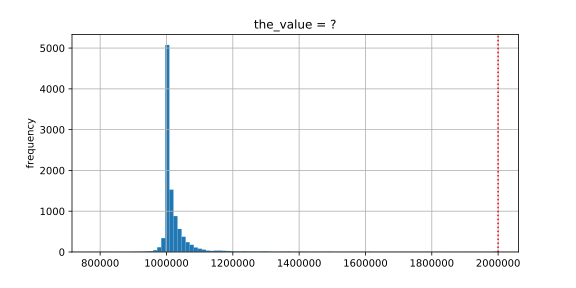
\includegraphics[width=1.1\textwidth]{../sync/parallel-add-histogram}
\end{frame}

\begin{frame}{but how?}
    \begin{itemize}
    \item probably not possible on single core
        \begin{itemize}
            \item exceptions can't occur in the middle of \texttt{add} instruction
        \end{itemize}
    \item \ldots but `add to memory' implemented with multiple steps
        \begin{itemize}
        \item still needs to load, add, store internally
        \item can be interleaved with what other cores do
        \end{itemize}
        \vspace{.5cm}
    \item<2-> {\small (and actually it's more complicated than that --- we'll talk later)}
    \end{itemize}
\end{frame}



\subsection{what is atomic?}

\begin{frame}{so, what is actually atomic}
    \begin{itemize}
    \item for now we'll assume: load/stores of `words' 
        \begin{itemize}
        \item  (64-bit machine = 64-bits words)
        \end{itemize}
        \vspace{.5cm}
    \item in general: \myemph{processor designer will tell you}
    \item their job to design caches, etc. to work as documented
    \end{itemize}
\end{frame}


\section{definitions: mutual exclusion, critical section}
\begin{frame}{some definitions}
\begin{itemize}
\item \textbf{mutual exclusion}: ensuring only one thread does a particular thing at a time
    \begin{itemize}
        \item like updating shared balance
    \end{itemize}
\item<2-> \textbf{critical section}: code that exactly one thread can execute at a time
    \begin{itemize}
        \item result of mutual exclusion
    \end{itemize}
\item<3-> \textbf{lock}: object only one thread can hold at a time
    \begin{itemize}
        \item interface for creating critical sections
    \end{itemize}
\end{itemize}
\end{frame}


\section{read-modify-write atomic operations}
\begin{frame}{atomic read-modfiy-write}
    \begin{itemize}
    \item really hard to build locks for atomic load store
        \begin{itemize}
        \item and normal load/stores aren't even atomic\ldots
        \end{itemize}
    \item \ldots so processors provide \myemph{read/modify/write} operations
        \vspace{.5cm}
    \item one instruction that\\\textit{atomically}\\reads \textit{and} modifies \textit{and} writes back a value
    \end{itemize}
\end{frame}

\subsection{x86 atomic exchange} 
\begin{frame}[fragile,label=atomicXchg]{x86 atomic exchange}
\begin{lstlisting}[language=myasm]
lock xchg (%ecx), %eax
\end{lstlisting}
\begin{itemize}
    \item atomic exchange
    \item \texttt{temp $\leftarrow$ M[ECX]}
    \item \texttt{M[ECX] $\leftarrow$ EAX}
    \item \texttt{EAX $\leftarrow$ temp}
    \item \ldots without being interrupted by other processors, etc.
\end{itemize}
\end{frame}


\begin{frame}{implementing atomic exchange}
    \begin{itemize}
    \item make sure other processors don't have cache block
    \item do read+modify+write operation
    \vspace{.5cm}
    \item recall: Modified state = ``I am the only one with a copy''
    \end{itemize}
\end{frame}



\section{locks}
\begin{frame}{lock analogy}
    \begin{itemize}
    \item agreement: whoever holds the flag can access shared resource
        \begin{itemize}
        \item flag doesn't actually do anything by itself\ldots
        \end{itemize}
    \item acquire/lock $\approx$ wait for and grab flag from table
    \item release/unlock $\approx$ put flag back on table
    \vspace{.5cm}
    \item<2-> agreement is \myemph{voluntary}
        \begin{itemize}
        \item thread tries to manipulate shared resource without lock? \\
            lock won't stop it\ldots
        \end{itemize}
    \item<2-> lock is \textit{held} by particular thread
    \end{itemize}
\end{frame}

% FIXME: lock analogy: hat
\begin{frame}[fragile,label=lockDefn]{the lock primitive}
    \begin{itemize}
    \item locks: an object with (at least) two operations:
        \begin{itemize}
        \item \textit{acquire} or \textit{lock} --- wait until lock is free, then ``grab'' it
        \item \textit{release} or \textit{unlock} --- let others use lock, wakeup waiters
        \end{itemize}
    \item typical usage: everyone acquires lock before using shared resource
        \begin{itemize}
        \item forget to acquire lock? weird things happen
        \end{itemize}
    \end{itemize}
\begin{lstlisting}[language=C++,style=small]
Lock(MilkLock);
if (no milk) {
    buy milk
}
Unlock(MilkLock);
\end{lstlisting}
\end{frame}

\begin{frame}[fragile,label=pthreadMutex]{pthread mutex}
\begin{lstlisting}[language=C++,style=small]
#include <pthread.h>

pthread_mutex_t MilkLock;
pthread_mutex_init(&MilkLock, NULL);
    // or: pthread_mutex_t MilkLock =
    //              PTHREAD_MUTEX_INITIALIZER;
...
pthread_mutex_lock(&MilkLock);
if (no milk) {
    buy milk
}
pthread_mutex_unlock(&MilkLock);
\end{lstlisting}
\end{frame}


\subsection{exercise}
\begin{frame}[fragile,label=lockEx]{exercise}
    \vspace{-0.5cm}
\begin{lstlisting}[style=smaller]
pthread_mutex_t lock1 = PTHREAD_MUTEX_INITIALIZER;
pthread_mutex_t lock2 = PTHREAD_MUTEX_INITIALIZER;
string one = "init one", two = "init two";
void ThreadA() {
    pthread_mutex_lock(&lock1);
    one = "one in ThreadA";  // (A1)
    pthread_mutex_unlock(&lock1);
    pthread_mutex_lock(&lock2);
    two = "two in ThreadA";  // (A2)
    pthread_mutex_unlock(&lock2);
}
void ThreadB() {
    pthread_mutex_lock(&lock1);
    one = "one in ThreadB";  // (B1)
    pthread_mutex_lock(&lock2);
    two = "two in ThreadB";  // (B2)
    pthread_mutex_unlock(&lock2);
    pthread_mutex_unlock(&lock1);
}
\end{lstlisting}
possible values of one/two after A+B run?
\end{frame}

\begin{frame}<0>[fragile,label=lockExSln]{solution}
\begin{itemize}
\item B1+A2
    \begin{itemize}
    \item A: L(1) A1 U(1) L
    \item B: L(1) B1 L(2) B2 U(2) U(1)
    \item A: L(2) A2 U(2)
    \end{itemize}
\item NOT A1+B2
    \begin{itemize}
    \item would need to run B1 before A1 before A2 before B2
    \item not possible because Lock1 held for entire B1+B2 operation
    \item so cannot fit A1+A2 in between B1 and B2
    \end{itemize}
\end{itemize}
\end{frame}

\iftoggle{heldback}{}{\againframe<1>{lockExSln}}

\begin{frame}[fragile,label=lockExAlt1]{exercise (alternate 1)}
    \vspace{-0.5cm}
\begin{lstlisting}[style=smaller]
pthread_mutex_t lock1 = PTHREAD_MUTEX_INITIALIZER;
pthread_mutex_t lock2 = PTHREAD_MUTEX_INITIALIZER;
string one = "init one", two = "init two";
void ThreadA() {
    pthread_mutex_lock(&lock2);
    two = "two in ThreadA";  // (A2)
    pthread_mutex_unlock(&lock2);
    pthread_mutex_lock(&lock1);
    one = "one in ThreadA";  // (A1)
    pthread_mutex_unlock(&lock1);
}
void ThreadB() {
    pthread_mutex_lock(&lock1);
    one = "one in ThreadB";  // (B1)
    pthread_mutex_lock(&lock2);
    two = "two in ThreadB";  // (B2)
    pthread_mutex_unlock(&lock2);
    pthread_mutex_unlock(&lock1);
}
\end{lstlisting}
possible values of one/two after A+B run?
\end{frame}

\begin{frame}[fragile,label=lockExAlt2]{exercise (alternate 2)}
    \vspace{-0.5cm}
\begin{lstlisting}[style=smaller]
pthread_mutex_t lock1 = PTHREAD_MUTEX_INITIALIZER;
pthread_mutex_t lock2 = PTHREAD_MUTEX_INITIALIZER;
string one = "init one", two = "init two";
void ThreadA() {
    pthread_mutex_lock(&lock2);
    two = "two in ThreadA";  // (A2)
    pthread_mutex_unlock(&lock2);
    pthread_mutex_lock(&lock1);
    one = "one in ThreadA";  // (A1)
    pthread_mutex_unlock(&lock1);
}
void ThreadB() {
    pthread_mutex_lock(&lock1);
    one = "one in ThreadB";  // (B1)
    pthread_mutex_unlock(&lock1);
    pthread_mutex_lock(&lock2);
    two = "two in ThreadB";  // (B2)
    pthread_mutex_unlock(&lock2);
}
\end{lstlisting}
possible values of one/two after A+B run?
\end{frame}


\subsection{pthread\_mutex: lock where you unlock}
\begin{frame}{POSIX mutex restrictions}
\begin{itemize}
\item pthread\_mutex rule: \myemph{unlock from same thread you lock in}
\vspace{.5cm}
\item implementation I gave before --- not a problem
\item \ldots but there other ways to implement mutexes
    \begin{itemize}
    \item e.g. might involve comparing with ``holding'' thread ID
    \end{itemize}
\end{itemize}
\end{frame}


\section{preview: beyond locks}
\begin{frame}{are locks enough?}
\begin{itemize}
    \item do we need more than locks?
\end{itemize}
\end{frame}

\begin{frame}{example 1: pipes?}
\begin{itemize}
\item suppose we want to implement a pipe with threads
\item \texttt{read} sometimes needs to wait for a \texttt{write}
\item don't want busy-wait
\begin{itemize}
\item (and trick of having writer unlock() so reader can finish a lock() is illegal)
\end{itemize}
\end{itemize}
\end{frame}

\begin{frame}{more synchronization primitives}
    \begin{itemize}
    \item need other ways to wait for threads to finish
    \item we'll introduce several synchronization ideas beyond locks:
        \begin{itemize}
        \item barriers --- (today)
        \item condition variables / monitors
        \item counting semaphores
        \item reader/writer locks
        \end{itemize}
    \end{itemize}
\end{frame}



\section{barriers}
\begin{frame}{barriers}
\begin{itemize}
\item compute minimum of 100M element array with 2 processors
\item algorithm:
\vspace{.5cm}
\item compute minimum of 50M of the elements on each CPU
    \begin{itemize}
    \item one thread for each CPU
    \end{itemize}
\item \myemph<2>{wait for all computations to finish}
\item take minimum of all the minimums
\end{itemize}
\end{frame}

\begin{frame}[fragile,label=barrierAPI]{barriers API}
\begin{itemize}
\item barrier.Initialize(NumberOfThreads)
\item barrier.Wait() --- return after all threads have waited
\vspace{.5cm}
\item idea: multiple threads perform computations in parallel
\item threads wait for \myemph{all other threads} to call Wait()
\end{itemize}
\end{frame}

\begin{frame}[fragile,label=barrierWait]{barrier: waiting for finish}
\begin{tikzpicture}
\node[label={north:Thread 0}] (code one) {
\begin{lstlisting}[language=C++,style=smaller]
partial_mins[0] = 
    /* min of first
       50M elems */;

barrier.Wait();


total_min = min(
    partial_mins[0],
    partial_mins[1]
);
\end{lstlisting}
};
\node[anchor=south] (code zero) at ([yshift=1cm]code one.north) {
\begin{lstlisting}[language=C++,style=smaller]
barrier.Initialize(2);
\end{lstlisting}
};

\node[label={north:Thread 1},anchor=north west] (code two) at ([xshift=1cm]code one.north east) {
\begin{lstlisting}[language=C++,style=smaller]


partial_mins[1] =
    /* min of last
       50M elems */
barrier.Wait();
\end{lstlisting}
};
\end{tikzpicture}
\end{frame}

\begin{frame}[fragile,label=barrierReuse]{barriers: reuse}
\begin{tikzpicture}
\node[label={north:Thread 0}] (code one) {
\begin{lstlisting}[
    language=C++,style=smaller,
    moredelim={**[is][\btHL<2|handout:0>]{@2}{2@}},
    moredelim={**[is][\btHL<3|handout:0>]{@3}{3@}},
    moredelim={**[is][\btHL<3|handout:0>]{@4}{4@}},
]
@2results[0][0]2@ = getInitial(0);
barrier.Wait();

@4results[1][0]4@ =
    computeFrom(0, 
        results[0][0],
        @3results[0][1]3@
    );
barrier.Wait();

results[2][0] =
    computeFrom(0,
        results[1][0],
        results[1][1]
    );
\end{lstlisting}
};
\node[label={north:Thread 1},anchor=north west] (code two) at ([xshift=1cm]code one.north east) {
\begin{lstlisting}[
    language=C++,style=smaller,
    moredelim={**[is][\btHL<2|handout:0>]{@2}{2@}},
    moredelim={**[is][\btHL<3|handout:0>]{@3}{3@}},
    moredelim={**[is][\btHL<3|handout:0>]{@4}{4@}},
]
@3results[0][1]3@ = getInitial(1);
barrier.Wait();

results[1][1] =
    computeFrom(1, 
        @2results[0][0],2@
        results[0][1]
    );
barrier.Wait();

results[2][1] =
    computeFrom(1,
        @4results[1][0]4@,
        results[1][1]
    );
\end{lstlisting}
};
\end{tikzpicture}
\end{frame}

\begin{frame}[fragile,label=pthreadBarrier]{pthread barriers}
\begin{lstlisting}[language=C++,style=smaller]
pthread_barrier_t barrier;
pthread_barrier_init(
    &barrier,
    NULL /* attributes */,
    numberOfThreads
);
...
...
pthread_barrier_wait(&barrier);
\end{lstlisting}
\end{frame}



\section{life HW}
\begin{frame}[fragile,label=lifeHW]{life homework (pseudocode)}
\begin{lstlisting}[
    language=C++,style=smaller,
    moredelim={**[is][\btHL<2|handout:0>]{@2}{2@}},
    moredelim={**[is][\btHL<3|handout:0>]{@3}{3@}},
    moredelim={**[is][\btHL<3|handout:0>]{@4}{4@}},
]
for (int time = 0; time < MAX_ITERATIONS; ++time) {
    for (int y = 0; y < size; ++y) {
        for (int x = 0; x < size; ++x) {
            to_grid(x, y) = computeValue(from_grid, x, y);
        }
    }
    swap(from_grid, to_grid);
}
\end{lstlisting}
\end{frame}

\begin{frame}{life homework}
\begin{itemize}
\item compute grid of values for time $t$ from grid for time $t-1$
    \begin{itemize}
    \item compute new value at $i,j$ based on surrounding values
    \end{itemize}
\vspace{.5cm}
\item parallel version: produce parts of grid in different threads
\item use barriers to finish time $t$ before going to time $t+1$
\end{itemize}
\end{frame}




\section{aside: reordering}

\section{revisiting atomicity}
\subsection{compiler reordering}
\begin{frame}[fragile,label=compReorder]{compilers move loads/stores (1)}
\begin{lstlisting}[language=C++,style=small,
    moredelim={**[is][\btHL<2|handout:2>]{@2}{2@}},
    moredelim={**[is][\btHL<3|handout:3>]{@3}{3@}},
    moredelim={**[is][\btHL<4|handout:4>]{@4}{4@}},
    moredelim={**[is][\btHL<5|handout:5>]{@5}{5@}},
]
void Alice() {
    note_from_alice = 1;
    @2do {} while (note_from_bob);2@
    if (no_milk) {++milk;}
}
\end{lstlisting}
\hrule
\begin{lstlisting}[language=myasm,style=smaller,
    moredelim={**[is][\btHL<2|handout:2>]{@2}{2@}},
    moredelim={**[is][\btHL<3|handout:3>]{@3}{3@}},
    moredelim={**[is][\btHL<4|handout:4>]{@4}{4@}},
    moredelim={**[is][\btHL<5|handout:5>]{@5}{5@}},
]
Alice:
  movl $1, note_from_alice  // note_from_alice <- 1
  movl note_from_bob, %eax  // eax <- note_from_bob
.L2:
  @2testl %eax, %eax2@
  @2jne .L22@                   // while (eax == 0) repeat
  cmpl $0, no_milk          // if (no_milk != 0) ...
  ...
\end{lstlisting}
\end{frame}

\begin{frame}[fragile,label=compReorder2]{compilers move loads/stores too (2)}
\begin{lstlisting}[language=C++,style=smaller,
    moredelim={**[is][\btHL<2|handout:2>]{@2}{2@}},
    moredelim={**[is][\btHL<3|handout:3>]{@3}{3@}},
    moredelim={**[is][\btHL<4|handout:4>]{@4}{4@}},
    moredelim={**[is][\btHL<5|handout:5>]{@5}{5@}},
]
void Alice() {
    @3note_from_alice = 1;3@  // "Alice waiting" signal for Bob()
    do {} while (note_from_bob);
    if (no_milk) {++milk;}
    @2note_from_alice = 2;2@
}
\end{lstlisting}
\hrule
\begin{lstlisting}[language=myasm,style=smaller,
    moredelim={**[is][\btHL<2|handout:2>]{@2}{2@}},
    moredelim={**[is][\btHL<3|handout:3>]{@3}{3@}},
    moredelim={**[is][\btHL<4|handout:4>]{@4}{4@}},
    moredelim={**[is][\btHL<5|handout:5>]{@5}{5@}},
]
Alice:  
  // compiler optimization: don't set note_from_alice to 1,
  // (why? it will be set to 2 anyway)
  @3movl note_from_bob, %eax3@  // eax <- note_from_bob
.L2:
  testl %eax, %eax          
  jne .L2                   // while (eax == 0) repeat
  ...
  @2movl $2, note_from_alice2@  // note_from_alice <- 2
\end{lstlisting}
\end{frame}


\subsection{processor reordering}
\begin{frame}[fragile,label=loadReorderSetup]{a simple race}
\begin{minipage}{0.45\textwidth}
\begin{lstlisting}[language=myasm,style=smaller]
thread_A:
    movl $1, x   /* x <- 1 */
    movl y, %eax /* return y */
    ret
\end{lstlisting}
\end{minipage}
\begin{minipage}{0.45\textwidth}
\begin{lstlisting}[language=myasm,style=smaller]
thread_B:
    movl $1, y   /* y <- 1 */
    movl x, %eax /* return x */
    ret
\end{lstlisting}
\end{minipage}
\\
\begin{lstlisting}[language=C++,style=smaller]
x = y = 0;
pthread_create(&A, NULL, thread_A, NULL);
pthread_create(&B, NULL, thread_B, NULL);
pthread_join(A, &A_result); pthread_join(B, &B_result);
printf("A:%d B:%d\n", (int) A_result, (int) B_result);
\end{lstlisting}
\begin{itemize}
\item<2-> if loads/stores atomic, then possible results:
    \begin{itemize}
    \item A:1 B:1 --- both moves into x and y, then both moves into eax execute
    \item A:0 B:1 --- thread A executes before thread B
    \item A:1 B:0 --- thread B executes before thread A
    \end{itemize}
\end{itemize}
\end{frame}

\begin{frame}[fragile,label=loadReorderExpResults]{a simple race: results}
\begin{minipage}{0.45\textwidth}
\begin{lstlisting}[language=myasm,style=smaller]
thread_A:
    movl $1, x   /* x <- 1 */
    movl y, %eax /* return y */
    ret
\end{lstlisting}
\end{minipage}
\begin{minipage}{0.45\textwidth}
\begin{lstlisting}[language=myasm,style=smaller]
thread_B:
    movl $1, y   /* y <- 1 */
    movl x, %eax /* return x */
    ret
\end{lstlisting}
\end{minipage}
\begin{lstlisting}[language=C++,style=smaller]
x = y = 0;
pthread_create(&A, NULL, thread_A, NULL);
pthread_create(&B, NULL, thread_B, NULL);
pthread_join(A, &A_result); pthread_join(B, &B_result);
printf("A:%d B:%d\n", (int) A_result, (int) B_result);
\end{lstlisting}
\vspace{-.5cm}
\begin{center}
\small my desktop, 100M trials: \\
\begin{tabular}{r|l|l}
frequency & result & ~ \\ \hline
$99\,823\,739$ & A:0 B:1 & (`A executes before B') \\
$171\,161$& A:1 B:0 & (`B executes before A') \\
$4\,706$ & A:1 B:1 & (`execute moves into x+y first') \\
\myemph<2>{$394$} & \myemph<2>{A:0 B:0} & \myemph<2>{???} \\
\end{tabular}
\end{center}
\end{frame}


\subsection{why reorder?}

\begin{frame}[fragile]{why reorder here?}
\begin{tikzpicture}
\node (thread A code) {
\begin{lstlisting}[language=myasm,style=smaller]
thread_A:
    movl $1, x   /* x <- 1 */
    movl y, %eax /* return y */
    ret
\end{lstlisting}
};
\node[anchor=north west] (thread B code) at ([xshift=.5cm]thread A code.north east) {
\begin{lstlisting}[language=myasm,style=smaller]
thread_B:
    movl $1, y   /* y <- 1 */
    movl x, %eax /* return x */
    ret
\end{lstlisting}
};
\end{tikzpicture}
\begin{itemize}
\item thread A: faster to load \texttt{y} right now!
\item \ldots rather than wait for write of \texttt{x} to finish
\end{itemize}
\end{frame}


\usetikzlibrary{calc}

\begin{frame}{why load/store reordering?}
\begin{itemize}
\item fast processor designs can execute instructions out of order
\item goal: do something instead of waiting for slow memory accesses, etc.
\item more on this later in the semester
\end{itemize}
\end{frame}





\section{pthreads and load/store reordering}
\begin{frame}{pthreads and reordering}
    \begin{itemize}
    \item many pthreads functions \myemph{prevent reordering}
        \begin{itemize}
        \item everything before function call actually happens before 
        \end{itemize}
    \item includes \myemph{preventing some optimizations}
        \begin{itemize}
        \item e.g. keeping global variable in register for too long
        \end{itemize}
    \vspace{.5cm}
    \item pthread\_mutex\_lock/unlock, pthread\_create, pthread\_join, \ldots
        \begin{itemize}
        \item basically: if pthreads is waiting for/starting something, no weird ordering
        \end{itemize}
    \item implementation part 1: prevent compiler reordering
    \item implementation part 2: use special instructions
        \begin{itemize}
        \item example: x86 \texttt{mfence} instruction
        \end{itemize}
    \end{itemize}
\end{frame}





\section{backup slides}
\begin{frame}{backup slides}
\end{frame}

\end{document}
